\documentclass{article}

\usepackage{graphicx}

\renewcommand{\labelenumii}{\theenumii}
\renewcommand{\theenumii}{\theenumi.\arabic{enumii}.}
\renewcommand{\theenumiii}{\theenumii\arabic{enumiii}.}


\begin{document}
\begin{figure}[t!]
	
\includegraphics[width= \linewidth]{PolimiLogo.png}
	\begin{center}
	Politecnico di Milano\\[4pt]
	AA 2018-2019  \\[4pt]
	Computer Science and Engineering \\[4pt]
	\begin{large}
	Software Engineering 2 Project
	\end{large}
	\end{center}
\end{figure}
\begin{flushright}
\begin{large}
Dalle Rive Fabio - 920082 \\[4pt]
Di Giacomantonio Marco - 846515 \\[4pt]
\end{large}
\end{flushright}
\newpage
{\Large\textbf{Table of Contents}}
	\begin{enumerate}
			\item Introduction
			\begin{enumerate}
				\item Purpose
				\item Scope
				\begin{enumerate}
					\item Description of the given problem
					\item Goals
				\end{enumerate}
				\item Definitions, Acronyms, Abbreviations
				\begin{enumerate}
					\item Definitions
					\item Acronyms
					\item Abbreviations
				\end{enumerate}
				\item Document structure
			\end{enumerate}
			\item Overall Description
			\begin{enumerate}
				\item Product perspective
				\item Product functions
				\begin{enumerate}
					\item Acquisition of users' data
					\item Company access to users' data
					\item Forwarding of following requests directly to the users and data anonymization
					\item AutomatedSOS
				\end{enumerate}
				\item User characteristics
				\item Assumptions, dependencies and constraints
				\begin{enumerate}
					\item Domain assumptions
				\end{enumerate}
			\end{enumerate}
			\item Specific requirements
			\begin{enumerate}
				\item External interface requirements	
				\begin{enumerate}
					\item Users interfaces
					\item Hardware interfaces
					\item Software interfaces
					\item Communication interfaces
				\end{enumerate}
				\item Scenarios
				\begin{enumerate}
					\item Scenario 1
					\item Scenario 2
					\item Scenario 3
				\end{enumerate}
				\item Functional requirements
				\begin{enumerate}
					\item Use case diagram
					\item Sequence diagram
				\end{enumerate}
				\item Performance requirements
				\item Design Constraints
				\begin{enumerate}
					\item Standard compliance
					\item Hardware limitation
					\item Other constraint
				\end{enumerate}
				\item Software system attributes
				\begin{enumerate}
					\item Reliability
					\item Security
					\item Maintainability
					\item Compatibility
				\end{enumerate}
			\end{enumerate}
			\item Formal Analysis Using Alloy
			\begin{enumerate}
				\item Alloy model
				\item World generated
				\item Alloy results
			\end{enumerate}
			\item Effort Spent
			\begin{enumerate}
			\item Dalle Rive Fabio
			\item Di Giacomantonio Marco
			\end{enumerate}
			\item Resources
			\item Revision History
	\end{enumerate}
	\newpage
\section{Introduction}
\subsection{Purpose}
The purpose of this project is to build a system, called Data4Help, that allows third parties to monitor the position and health status of users. The data are collected by TrackMe, the company that wants to develop Data4Help, and are shared with other companies which are interested in those data.
Furthermore, TrackMe wants to develop AutomatedSOS, a system build on top of Data4Help. AutomatedSOS is a service designed for elderly people, it is able to intervene by calling an ambulance if the health parameters of the user are below some fixed thresholds.
\subsection{Scope}
\subsubsection{Description of the given problem}
TrackMe is a company that wants to develop a software-based service allowing third parties to monitor the location and health status of users. This service is called Data4Help. The service supports the registration of the visitors who, by registering, allow TrackMe to acquire their data. Also it supports the registration of third parties. After registration, these third parties can request: 
\begin{itemize}
	\item Access to the data of some specific user.
	\item Access to anonymized data of groups of users.
\end{itemize}
TrackMe also wants to develop a non-intrusive SOS service for elderly people, called AutomatedSOS. AutomatedSOS is build on top of Data4Help. This service is designed to monitor health status of users and to send an ambulance to the location of the user if some parameters are below some specified thresholds. 
\subsubsection{Goals}
\begin{itemize}
	\item {[G1]} Visitor can become User after providing credentials.
	\item {[G2]} User can accept or reject the request of access to his data formulated by companies.
	\item {[G3]} If user's parameters are below specified thresholds, an ambulance is called within 5 seconds. 
	\begin{itemize}
		\item {[G3.1]} Ambulance is required at current user's location. 
	\end{itemize}
	\item {[G4]} Company can sign up as Company to Data4Help and AutomatedSOS. 
	\item {[G5]} Company can be recognized providing a password and vat number.
	\item {[G6]} Company can formulate a request to see anonymized data of a group of users.
	\item {[G7]} Company can formulate a request to see data of a specific user providing his SSN.
	\item {[G8]} Company can see anonymized data of a group of users.
	\item {[G9]} Company can see data of a specific user providing his SSN.
	\item {[G10]} Company can subscribe to users' new data.
	\item {[G11]} Data4Help can forward companies' requests to users. 
	\item {[G12]} A user of Data4Help becomes automatically a user of AutomateSOS if he is older than \emph{Age}.
\end{itemize} 
\subsection{Definitions, Acronyms, Abbreviations}
\subsubsection{Definitions}
\begin{itemize}
	\item\textbf{Visitor:} a person who still has to register to Data4Help and\\ AutomatedSOS.
	\item\textbf{User:} a person who is registered to Data4Help and AutomatedSOS.
	\item\textbf{Third Parties / Companies:} company.
	\item\textbf{Data:} User's monitored data: location + heart rate + calories burned + time spent exercising + step walked 
	\item \textbf{Threshold:} Flexible value related to the heart rate data acquired by the smart watch in which the system-to-be is installed. This value is computed by well-known equation that operate with user's data. Among the others it also depends of the kind of activity that a user is doing and his age.  
	\item \textbf{Subscribe to data:} A company which is subscribed to user's data or to users group's data, receives the requested data as soon as they are produced.  
	\item \textbf{Pendent user:} A user that a company want to follow but has not answered to the following request yet.
	\item \textbf{Single user request / Following request:} A formal request issued by a company to see the data of a user.
	\item \textbf{Group of users request:} A formal request issued by a company to see the data of a group of users.
	\item \textbf{Dandling request:} A single user request that has not already been approved by a user.
	\item \textbf{Age:} age over which a user is subscribed to AutomateSOS. 
	\item \textbf{Ambulance Service:} service which is offered by external components. AutomatedSOS will contact this service sharing the current location if a user if the user's heart rate is below the \emph{Threshold}.
	\item \textbf{Call Ambulance}: this term is used through the document has a short cut to: "AutomatedSOS issue a formal request for an ambulance at the current user location to the Ambulance Service".
\end{itemize}
\subsubsection{Acronyms}
\begin{itemize}
	\item RASD - Required Analysis and Specification Document
	\item GPS - Global Positioning System
	\item SSN - Social Security Number
\end{itemize}
\subsubsection{Abbreviations}
\begin{itemize}
	\item {[Gn]}: n-th goal
	\item {[Dn]}: n-th domain assumption
	\item {[Rn]}: n-th functional requirement
\end{itemize}
\subsection{Document structure}
\begin{description}
	\item [Introduction] gives an introduction to the problem and describe the purpose of Data4Help and AutomatedSOS. It also contains the goals that these systems-to-be must be able to deliver to users and third party companies.
	\item [Overall Description] gives an overview of the functions that the systems-to-be are able to deliver to users and third parties. In this section, users of the systems-to-be, are better identified, i.e. the kind of users that interact with Data4Help and AutomatedSOS. Assumptions used by Data4Help and AutomatedSOS are presented in this section. 
	\item [Specific Requirements] gives and overview of which functional requirements are needed to fulfill goals we already presented. Moreover it gives an overview of non-functional requirements.
	\item [Formal Analysis Using Alloy] includes the Alloy model and the discussion of its purpose. Also, a world generated by this model is shown.
	\item [Effort Spent] shows the effort spent by each group member while working on this project.
	\item [Resources] includes the reference documents. 
\end{description}
\newpage
\section{Overall Description}
\subsection{Product perspective}
Data4Help and AutomatedSOS are intended as a background application that are installed inside a smart watch. The systems-to-be acquire data of the users through the smart watch. A user register himself for Data4Help accessing the website page(https://www.data4help.com) that TrackMe provide for this application. Once a user is in the web page he can register himself to Data4Help typing the required information. During the registration process, the user will be required to type his Google or Apple account. This is meant to allow TrackMe to know which device a user has; and among those, let the user picks the one from which data will be acquired. Once a user subscribe to Data4Help, if he has an age that is greater or equal to \emph{Age} he will be automatically enrolled in AutomatedSOS.
\begin{figure}[h!]
\centering
    \textbf{}\par\medskip
	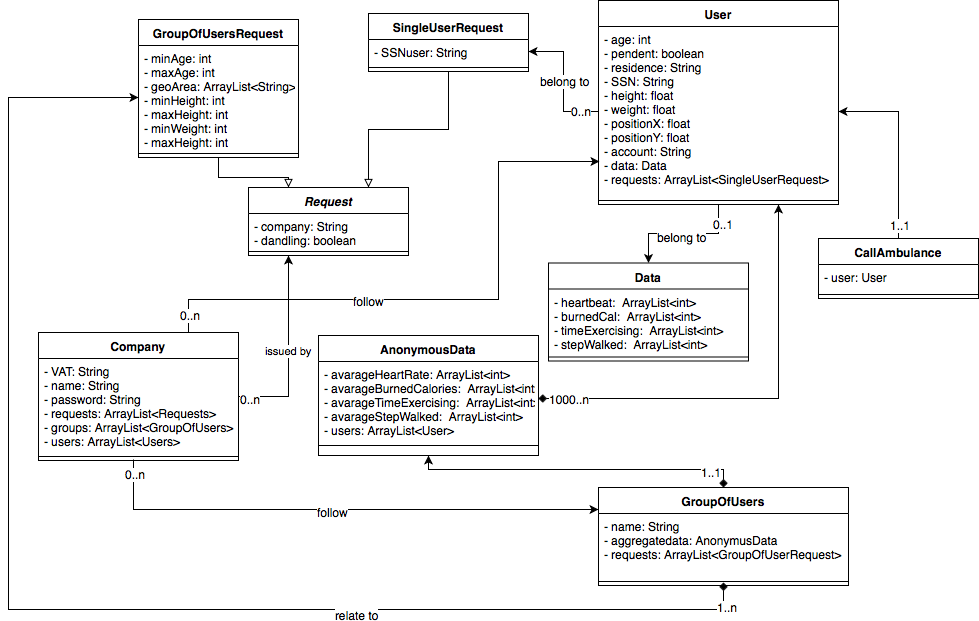
\includegraphics[width= \linewidth]{model.png}
\end{figure}
\subsection{Product functions}
Considering all the goals previously presented, we can sum up into four categories the main functions of the product: \newpage
\subsubsection{Acquisition of users' data}
The system-to-be runs on smart watches, assumed to be able to communicate the data directly to TrackMe's servers. It is also assumed that these smart watches have GPS integrated in their hardware. It means that this product works only with smart watches that have a direct internet connection(they have an integrated SIM card). Future updates will enable to use also smart watch that use Bluetooth to communicate data to a smart phone that then send data towards TrackMe servers.
\subsubsection{Company access to users' data}
The system-to-be enables companies to access data of a specific user or of groups of users. Companies access to these data through the web page(https//www.data4help.com). Data are shown in a user-friendly way. Some samples of the web page will be shown in the User Interface section.
\subsubsection{Forwarding of following requests directly to the users and data anonymization}
Companies are able to send following requests, in order to access user data. The system-to-be allows companies to issue request to users. Every time that a company request to access some data, a request is created and stored inside TrackMe's servers. Analizing the request, TrackMe's servers will decide how to proceed:\\
\begin{itemize}
\item If the request concerns a specific user, TrackMe sends an email to the user asking to accept or reject it.
\item If the request concerns a group of users(with more than 1000 user), create a group and anonymizes the corresponding data. 
\end{itemize}
\subsubsection{AutomatedSOS}
While registering Data4Help, the user is asked to submit his age. Basing on some creteria chosen from the managment, a value \emph{Age} for the age is chosen. If the user's age is greater than \emph{Age} AutomatedSOS is activated automatically. AutomatedSOS is a service that monitors the heartbeat of the user and if it's lower than \emph{Threshold}, calls an ambulance addressed to the user's position within 5 seconds. This is achieved by sharing the current user location(acquire through GPS integrated in the smart watch) with the external \emph{Ambulance Service}.
\subsection{User characteristics}
\begin{itemize}
\item \emph{Visitor}: a person not registered. The only thing he can do is proceeding with sing up.
\item \emph{User}: a person passed through a successful registration process. His data can be tracked, he can accept or reject compaines' following request.
 \item \emph{Company}: an entity that can be recognised as a company. It can see data of a specific user or anonimous data of a group of users. 
 \item \emph{TrackMe}: the whole hardware and software interfaces over which Data4Help and AutomatedSOS run.
\end{itemize}
\subsection{Assumption, dependencies and constraints}
\subsubsection{Domain assumptions}
\begin{itemize}
	\item {[D1]} The user's email is already known by TrackMe.
	\item {[D2]} Only real companies can sing up as companies.
	\item {[D3]}  At most 5 seconds are necessary to send user location and call an ambulance when parameters are below the threshold.
	\item {[D4]} Smart watch in which the system-to-be is installed have: \emph{GPS, Accelerometer, LTE, Photoplethysmography}.
	\item {[D5]} When the system shows the position of a user it means that the user is
actually there.
	\item {[D6]} During the registration process the user inserts all the requested data.
	\item {[D7]} The user has the physical characteristics that he inserted in the system.
	\item {[D8]} Companies have a name and a vat number. VAT number is unique.
	\item {[D9]} Companies know the SSN of the user.  
	\item {[D10]} Current user's residence is the CAP of user's residence. 
\end{itemize}\newpage
\section{Specific Requirements}
\subsection{External interface requirements}
\subsubsection{User interfaces}
In this section are presented some pictures that show how the web page https://www.data4help.com should look like after the deployment.
\begin{figure}[h!]
\centering
    \textbf{Homepage.}\par\medskip
	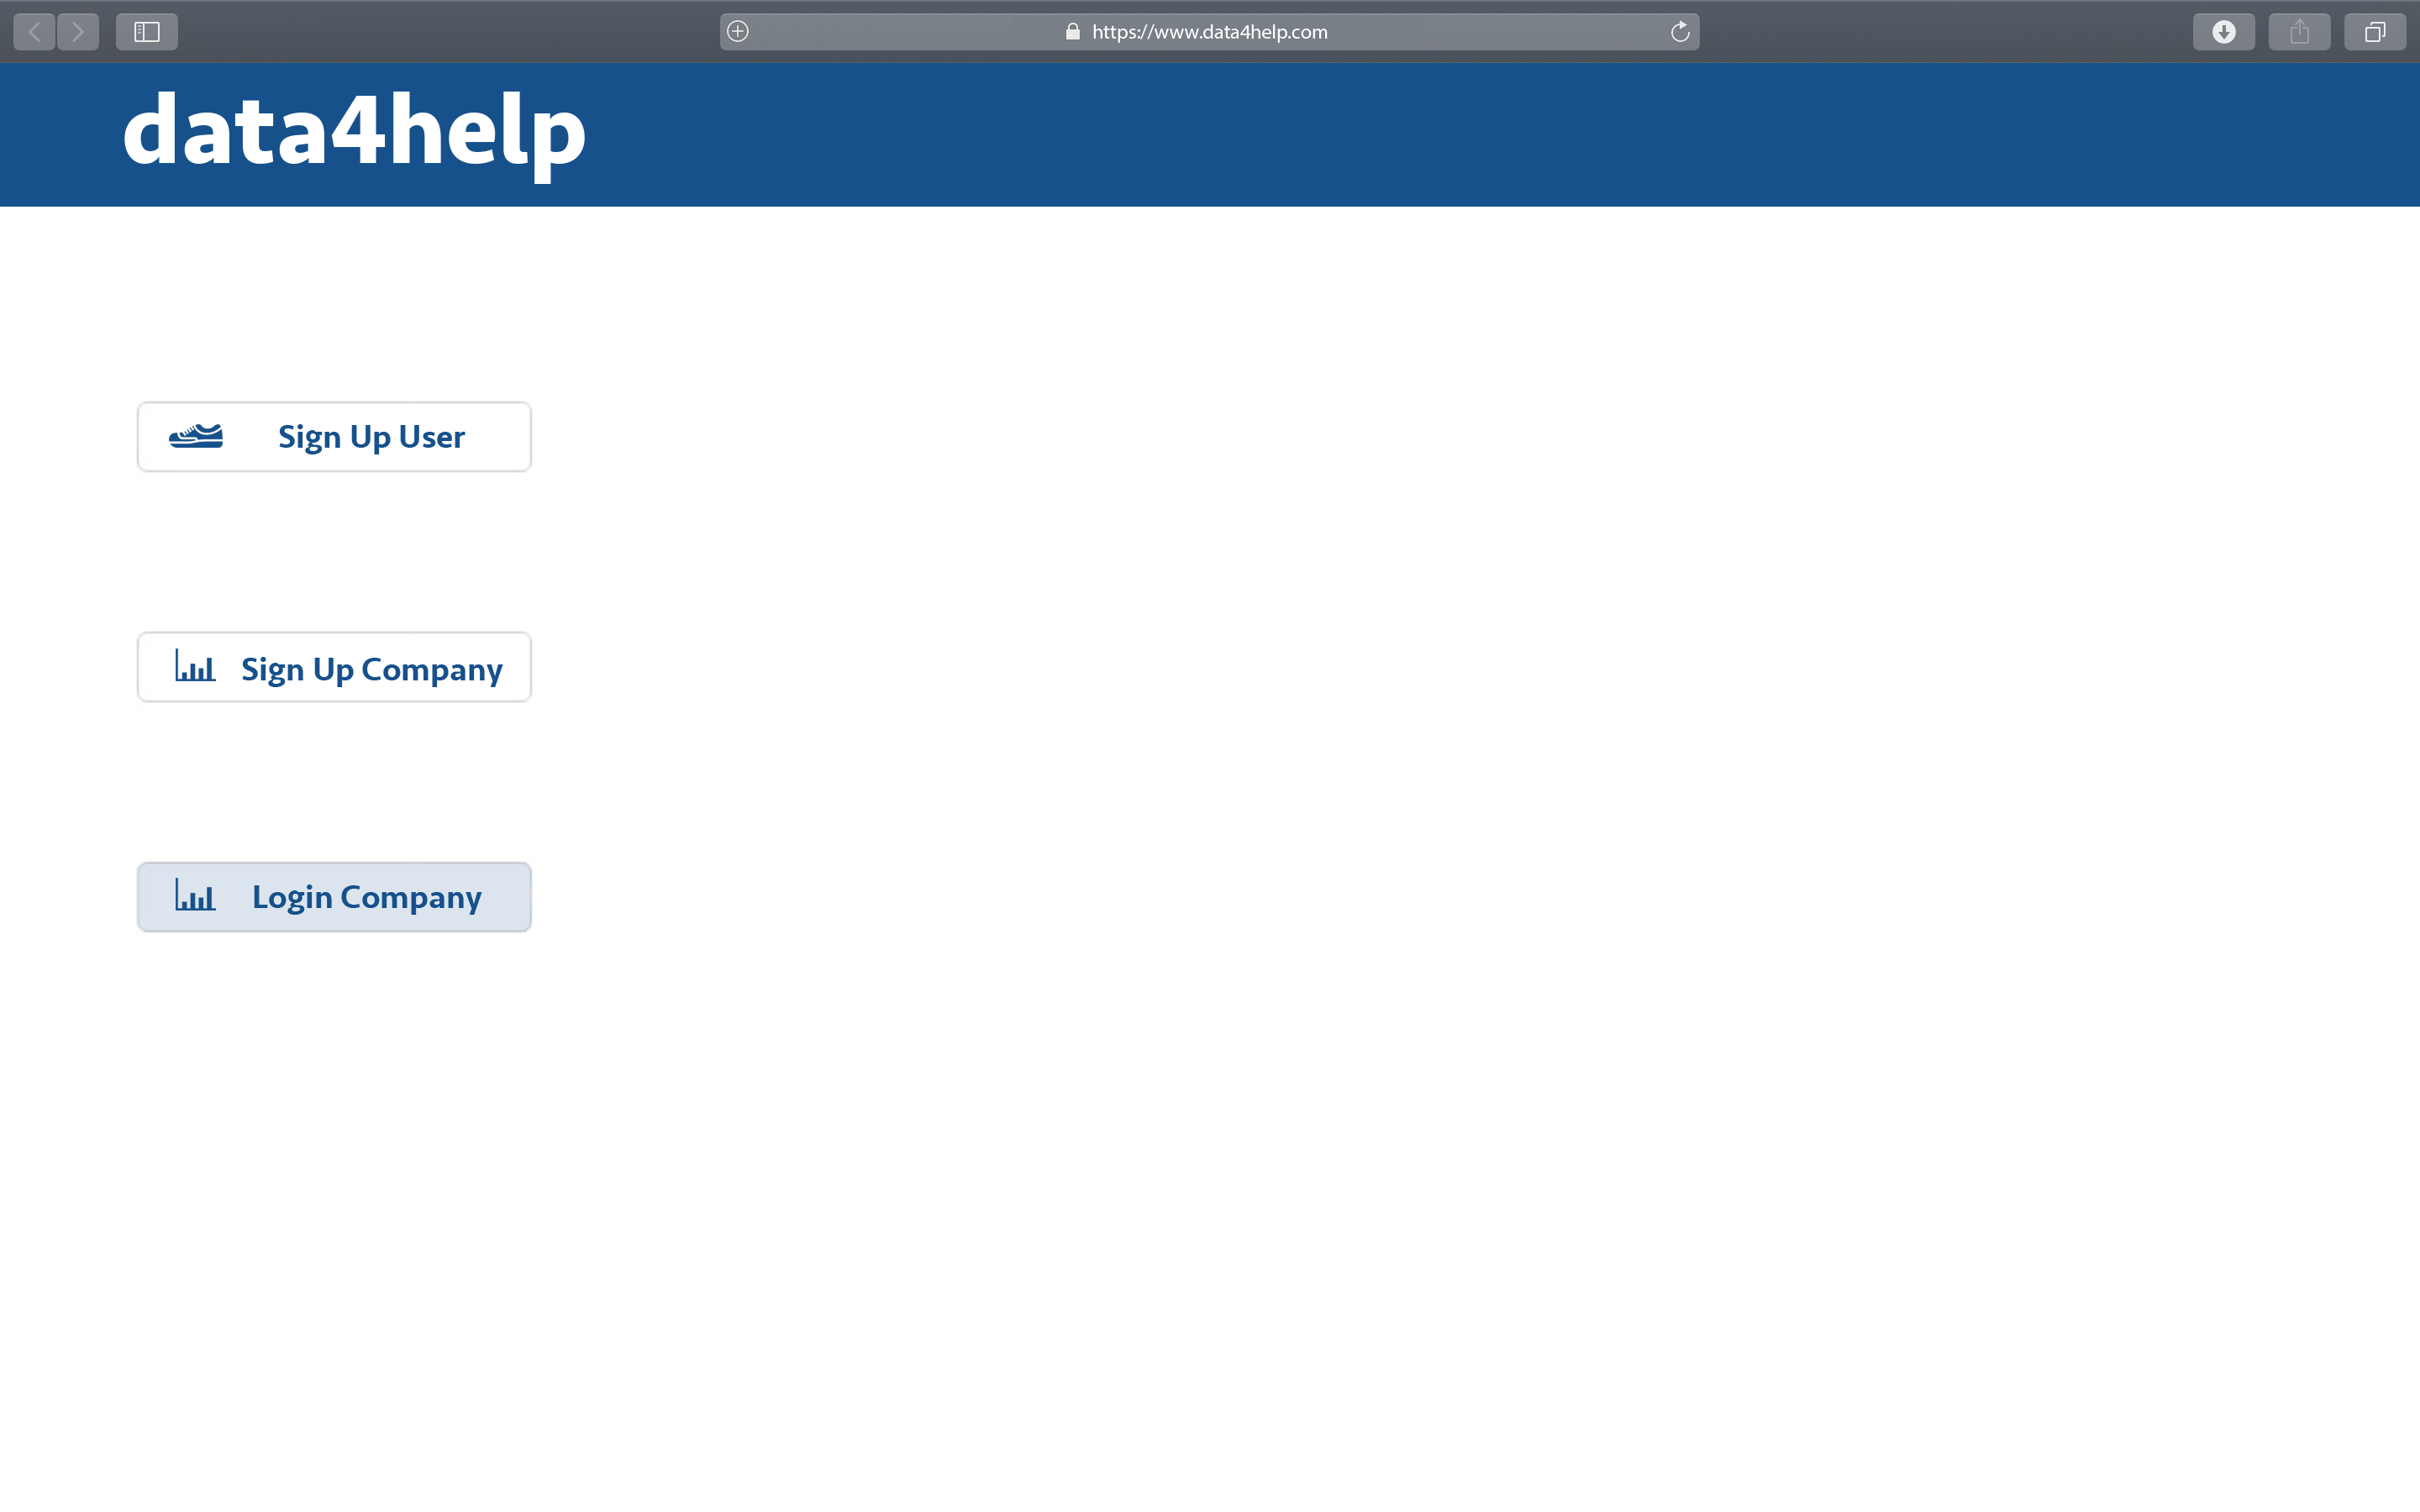
\includegraphics[width= \linewidth]{1homepage.png}
\end{figure}
\begin{figure}[h!]
\centering
    \textbf{User sign up.}\par\medskip
	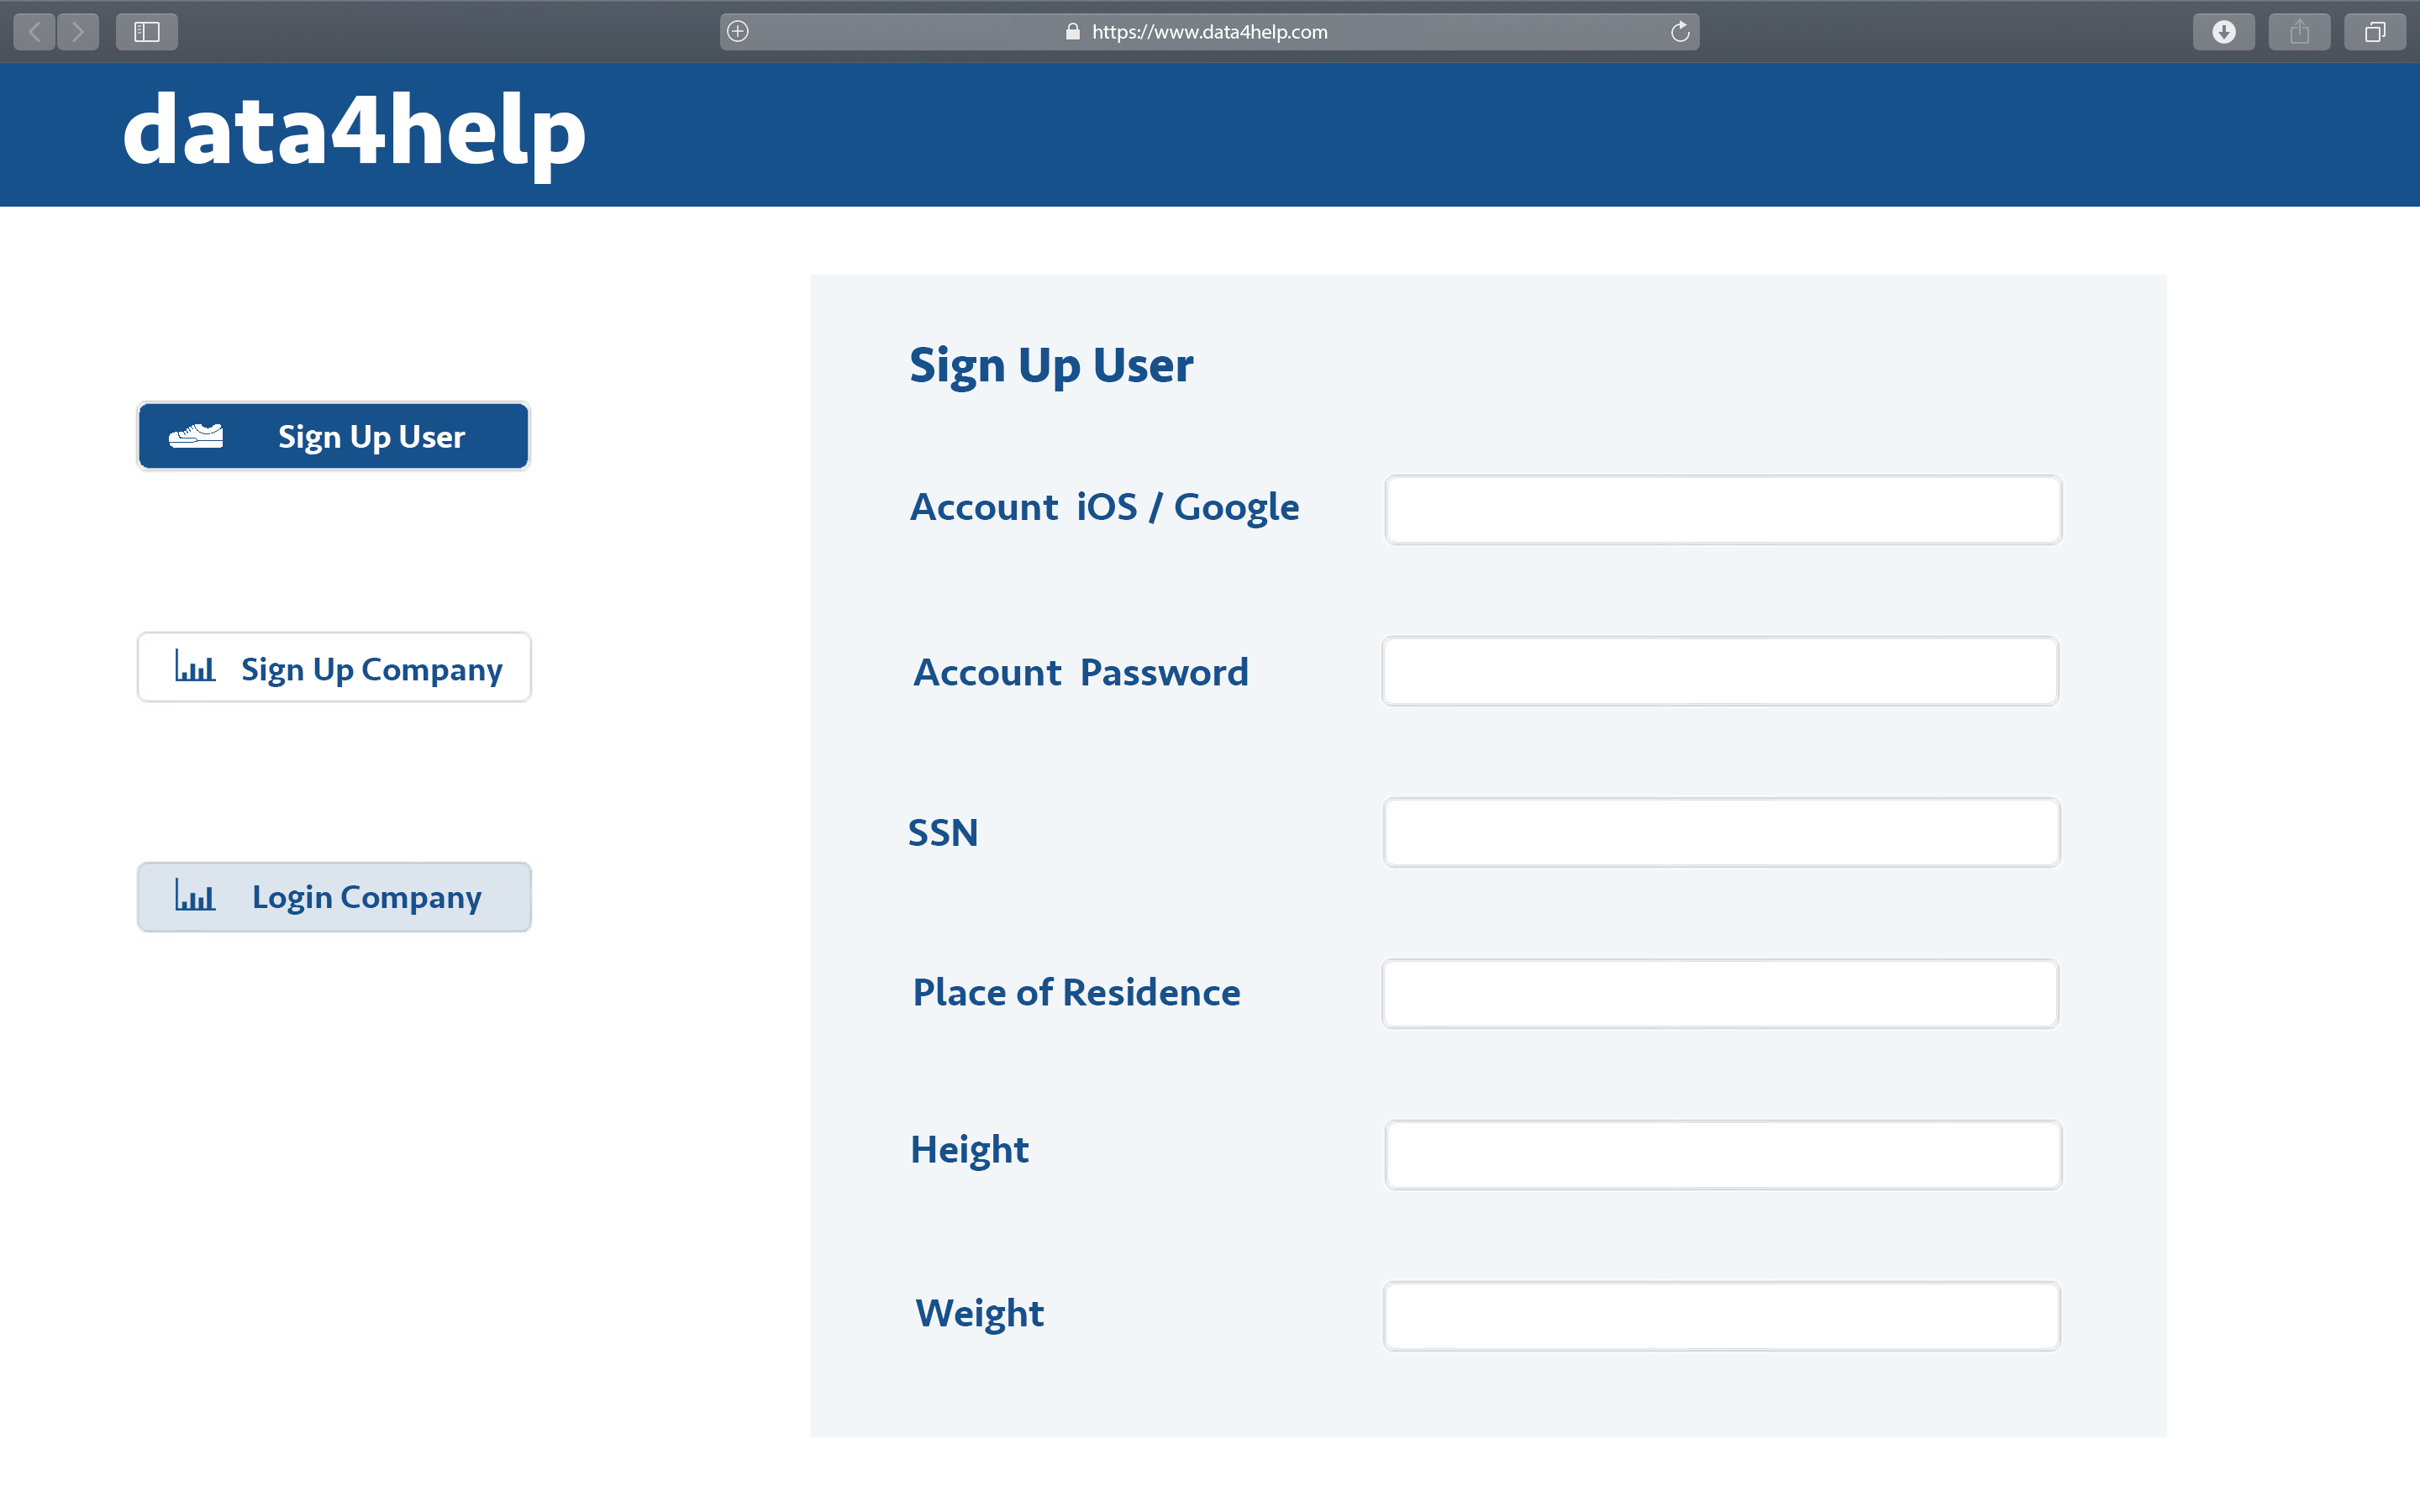
\includegraphics[width= \linewidth]{2signupuser.png}
\end{figure}\newpage
\begin{figure}[h!]
\centering
    \textbf{Company sing up.}\par\medskip
	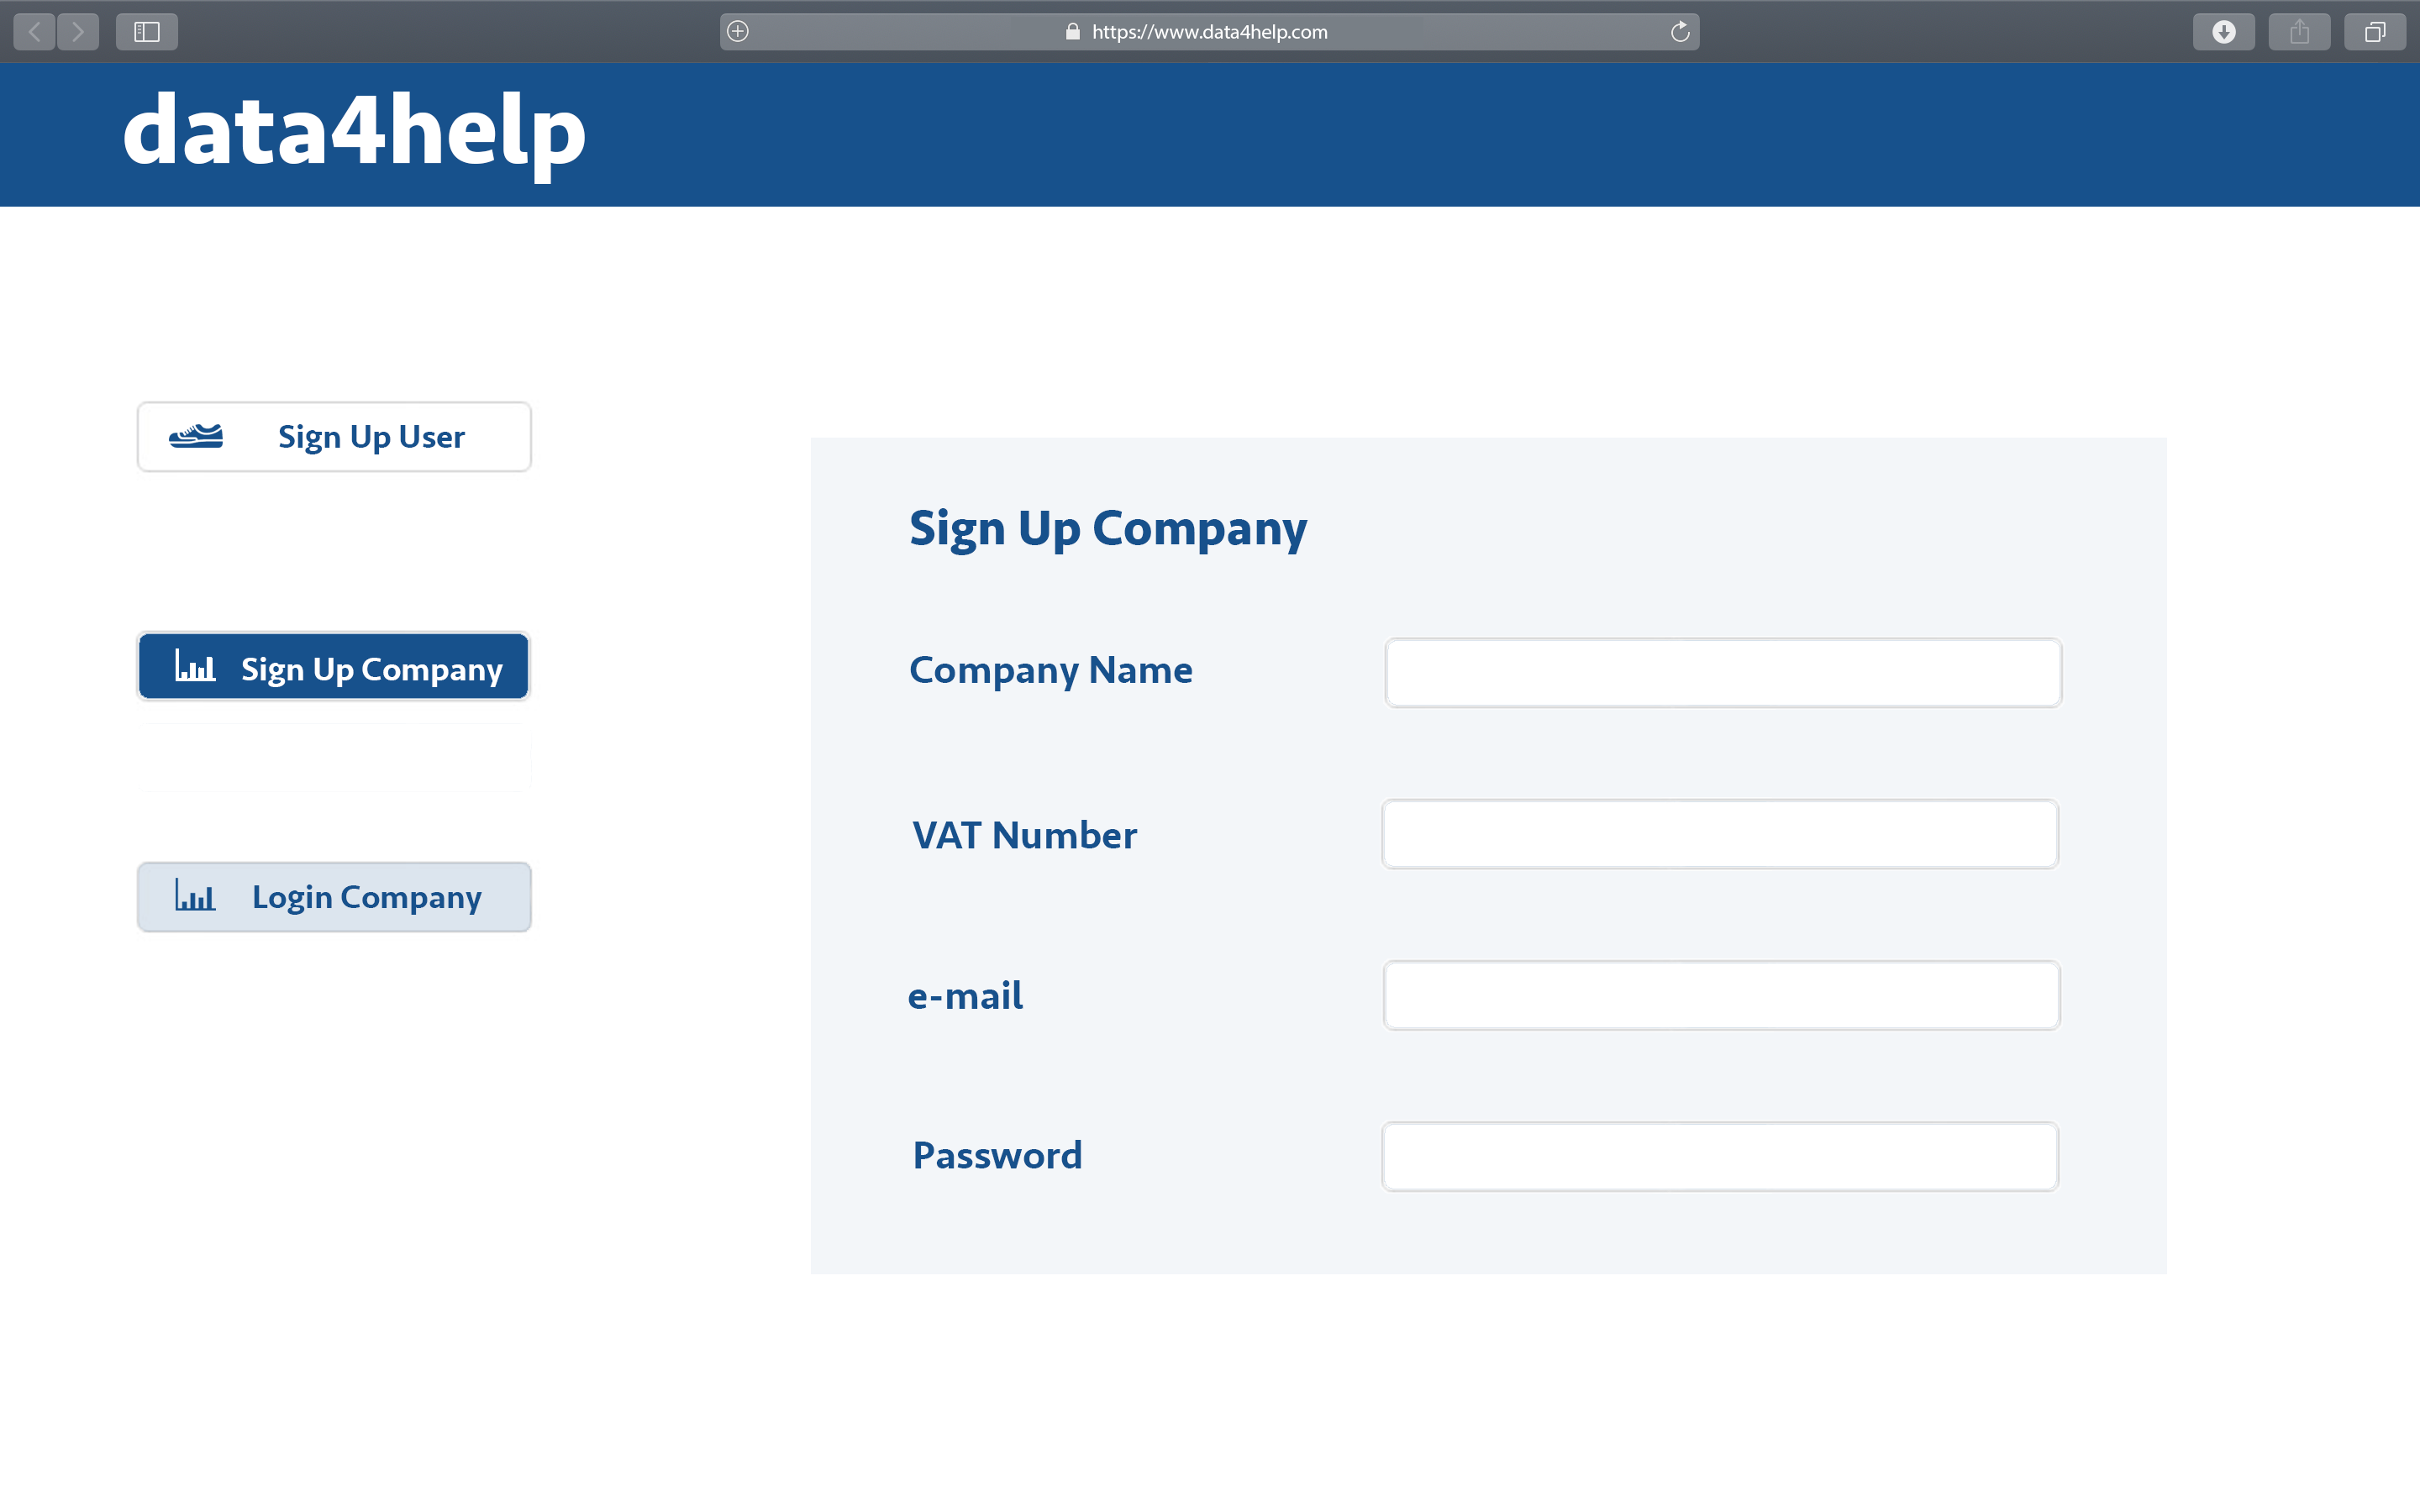
\includegraphics[width= \linewidth]{3signupcompany.png}
\end{figure}
\begin{figure}[h!]
\centering
    \textbf{Company login.}\par\medskip
	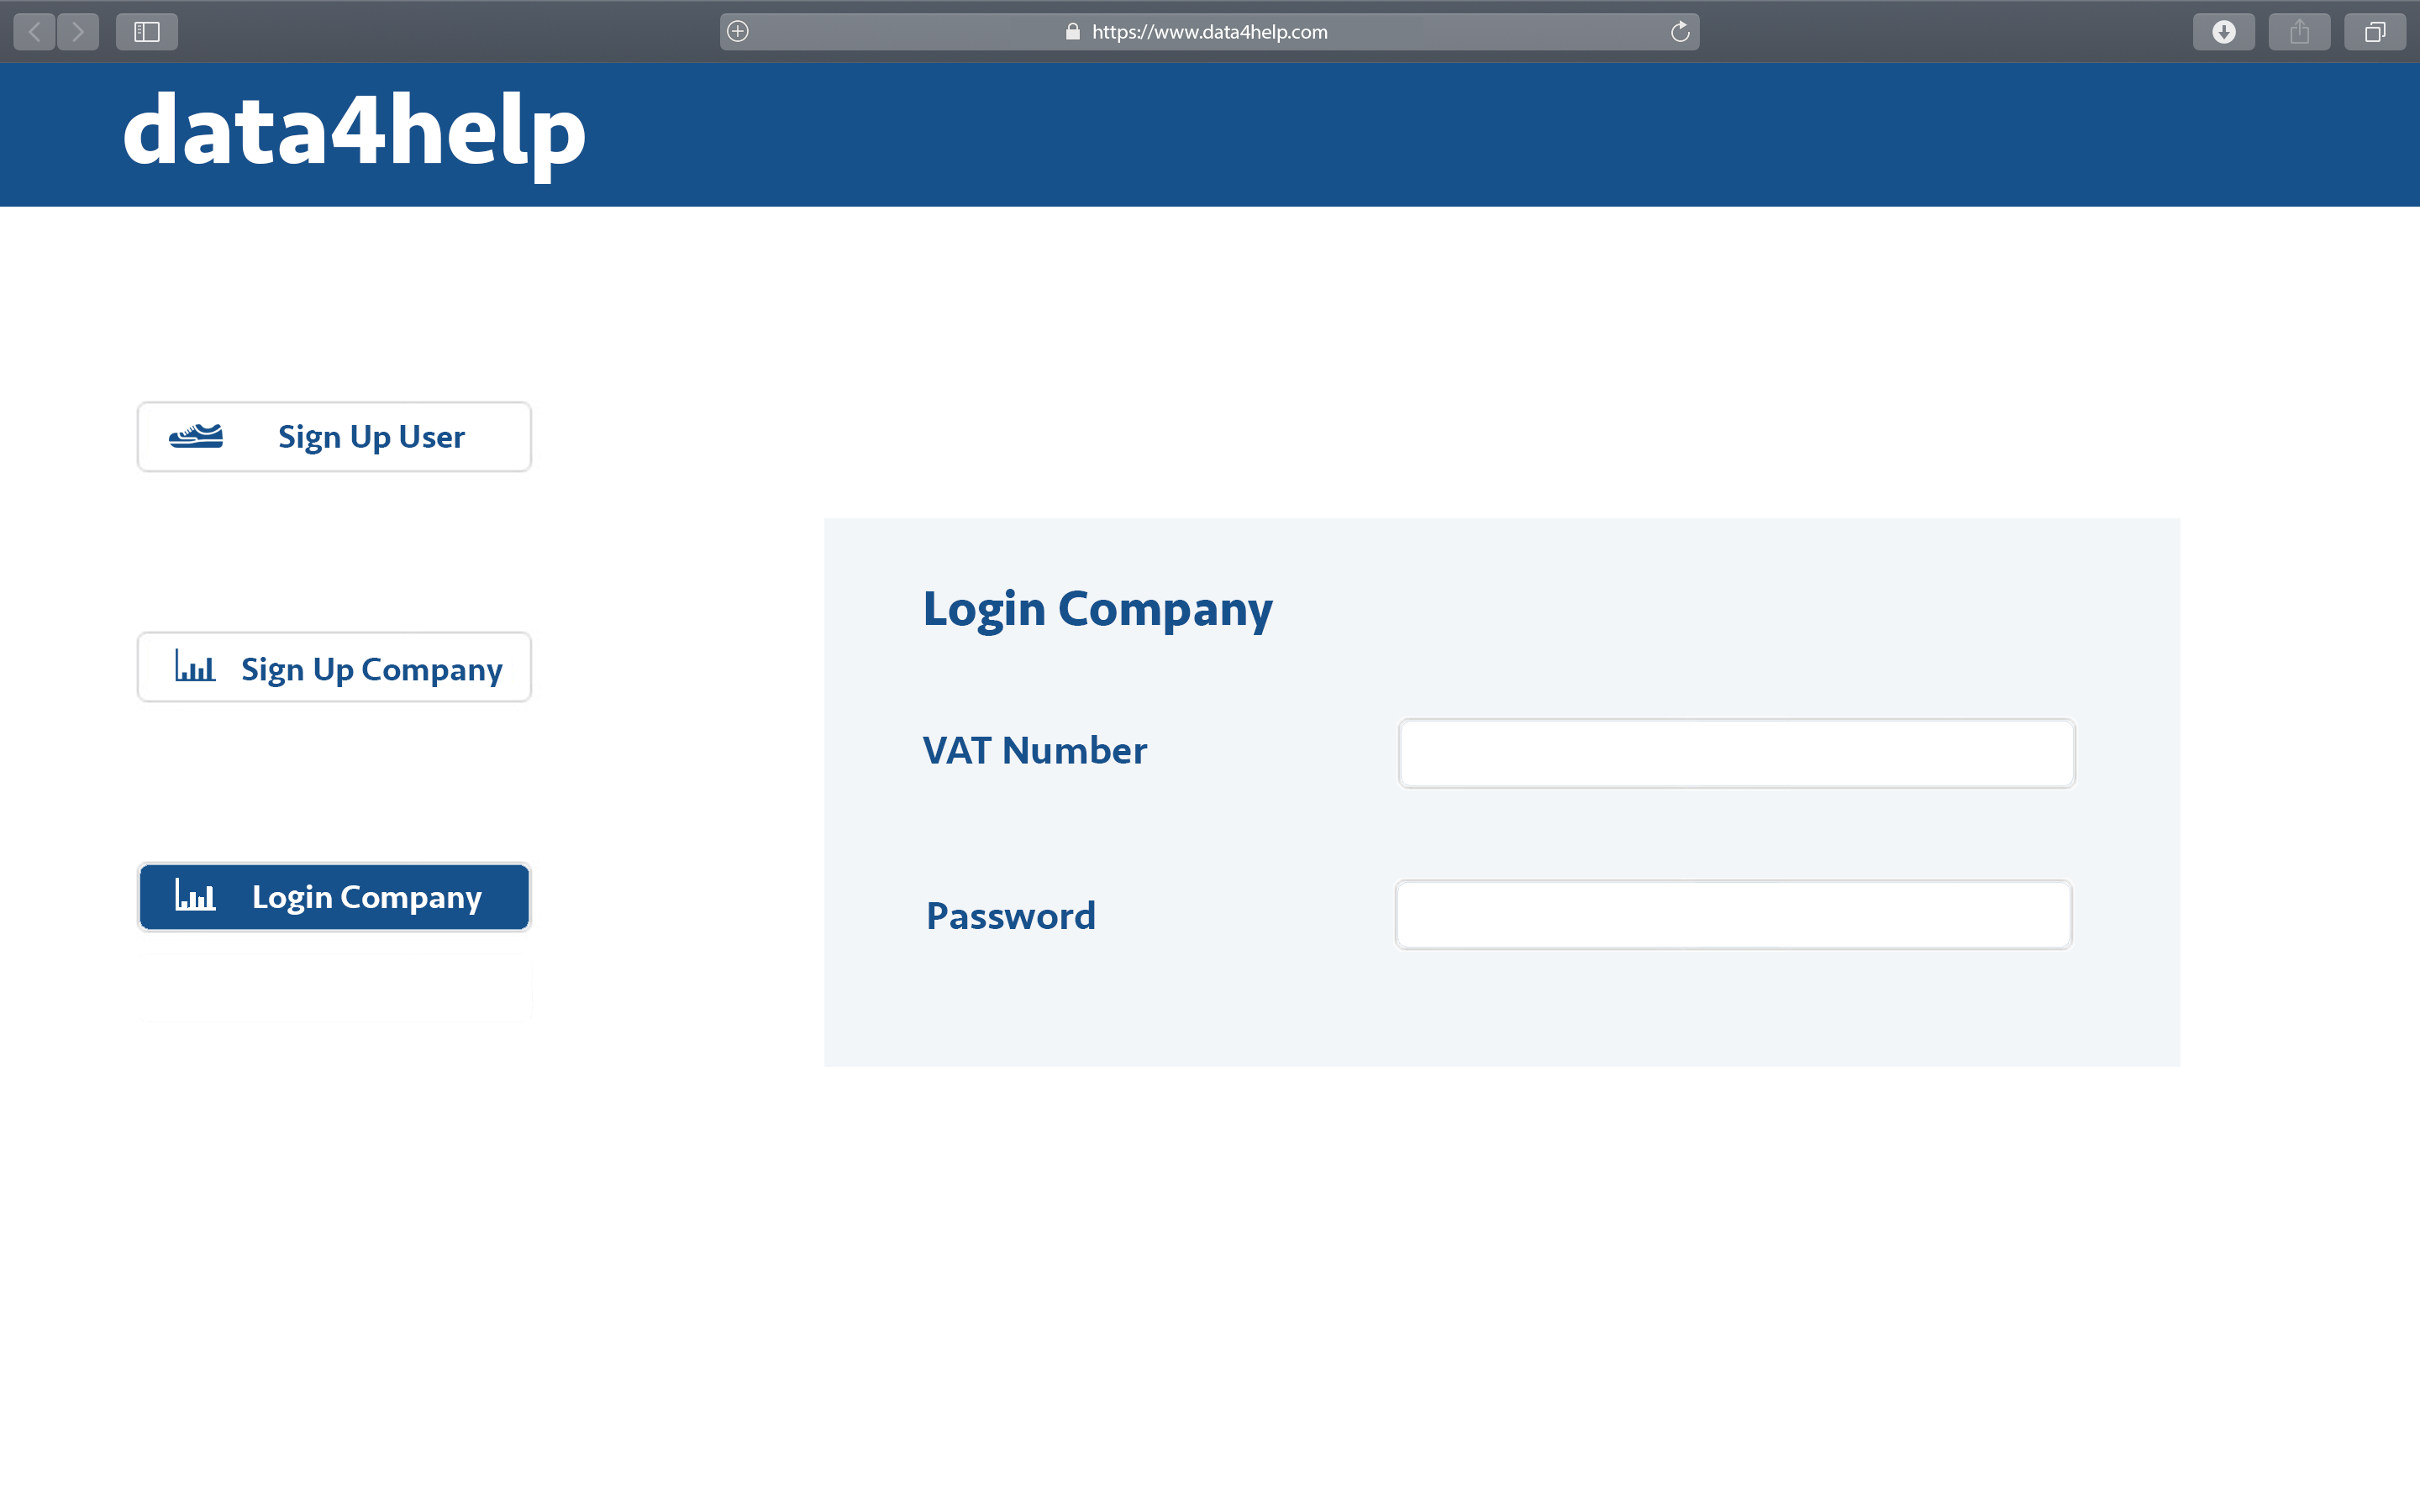
\includegraphics[width= \linewidth]{4logincompany.png}
\end{figure}\newpage
\begin{figure}[h!]
\centering
    \textbf{Requests.}\par\medskip
	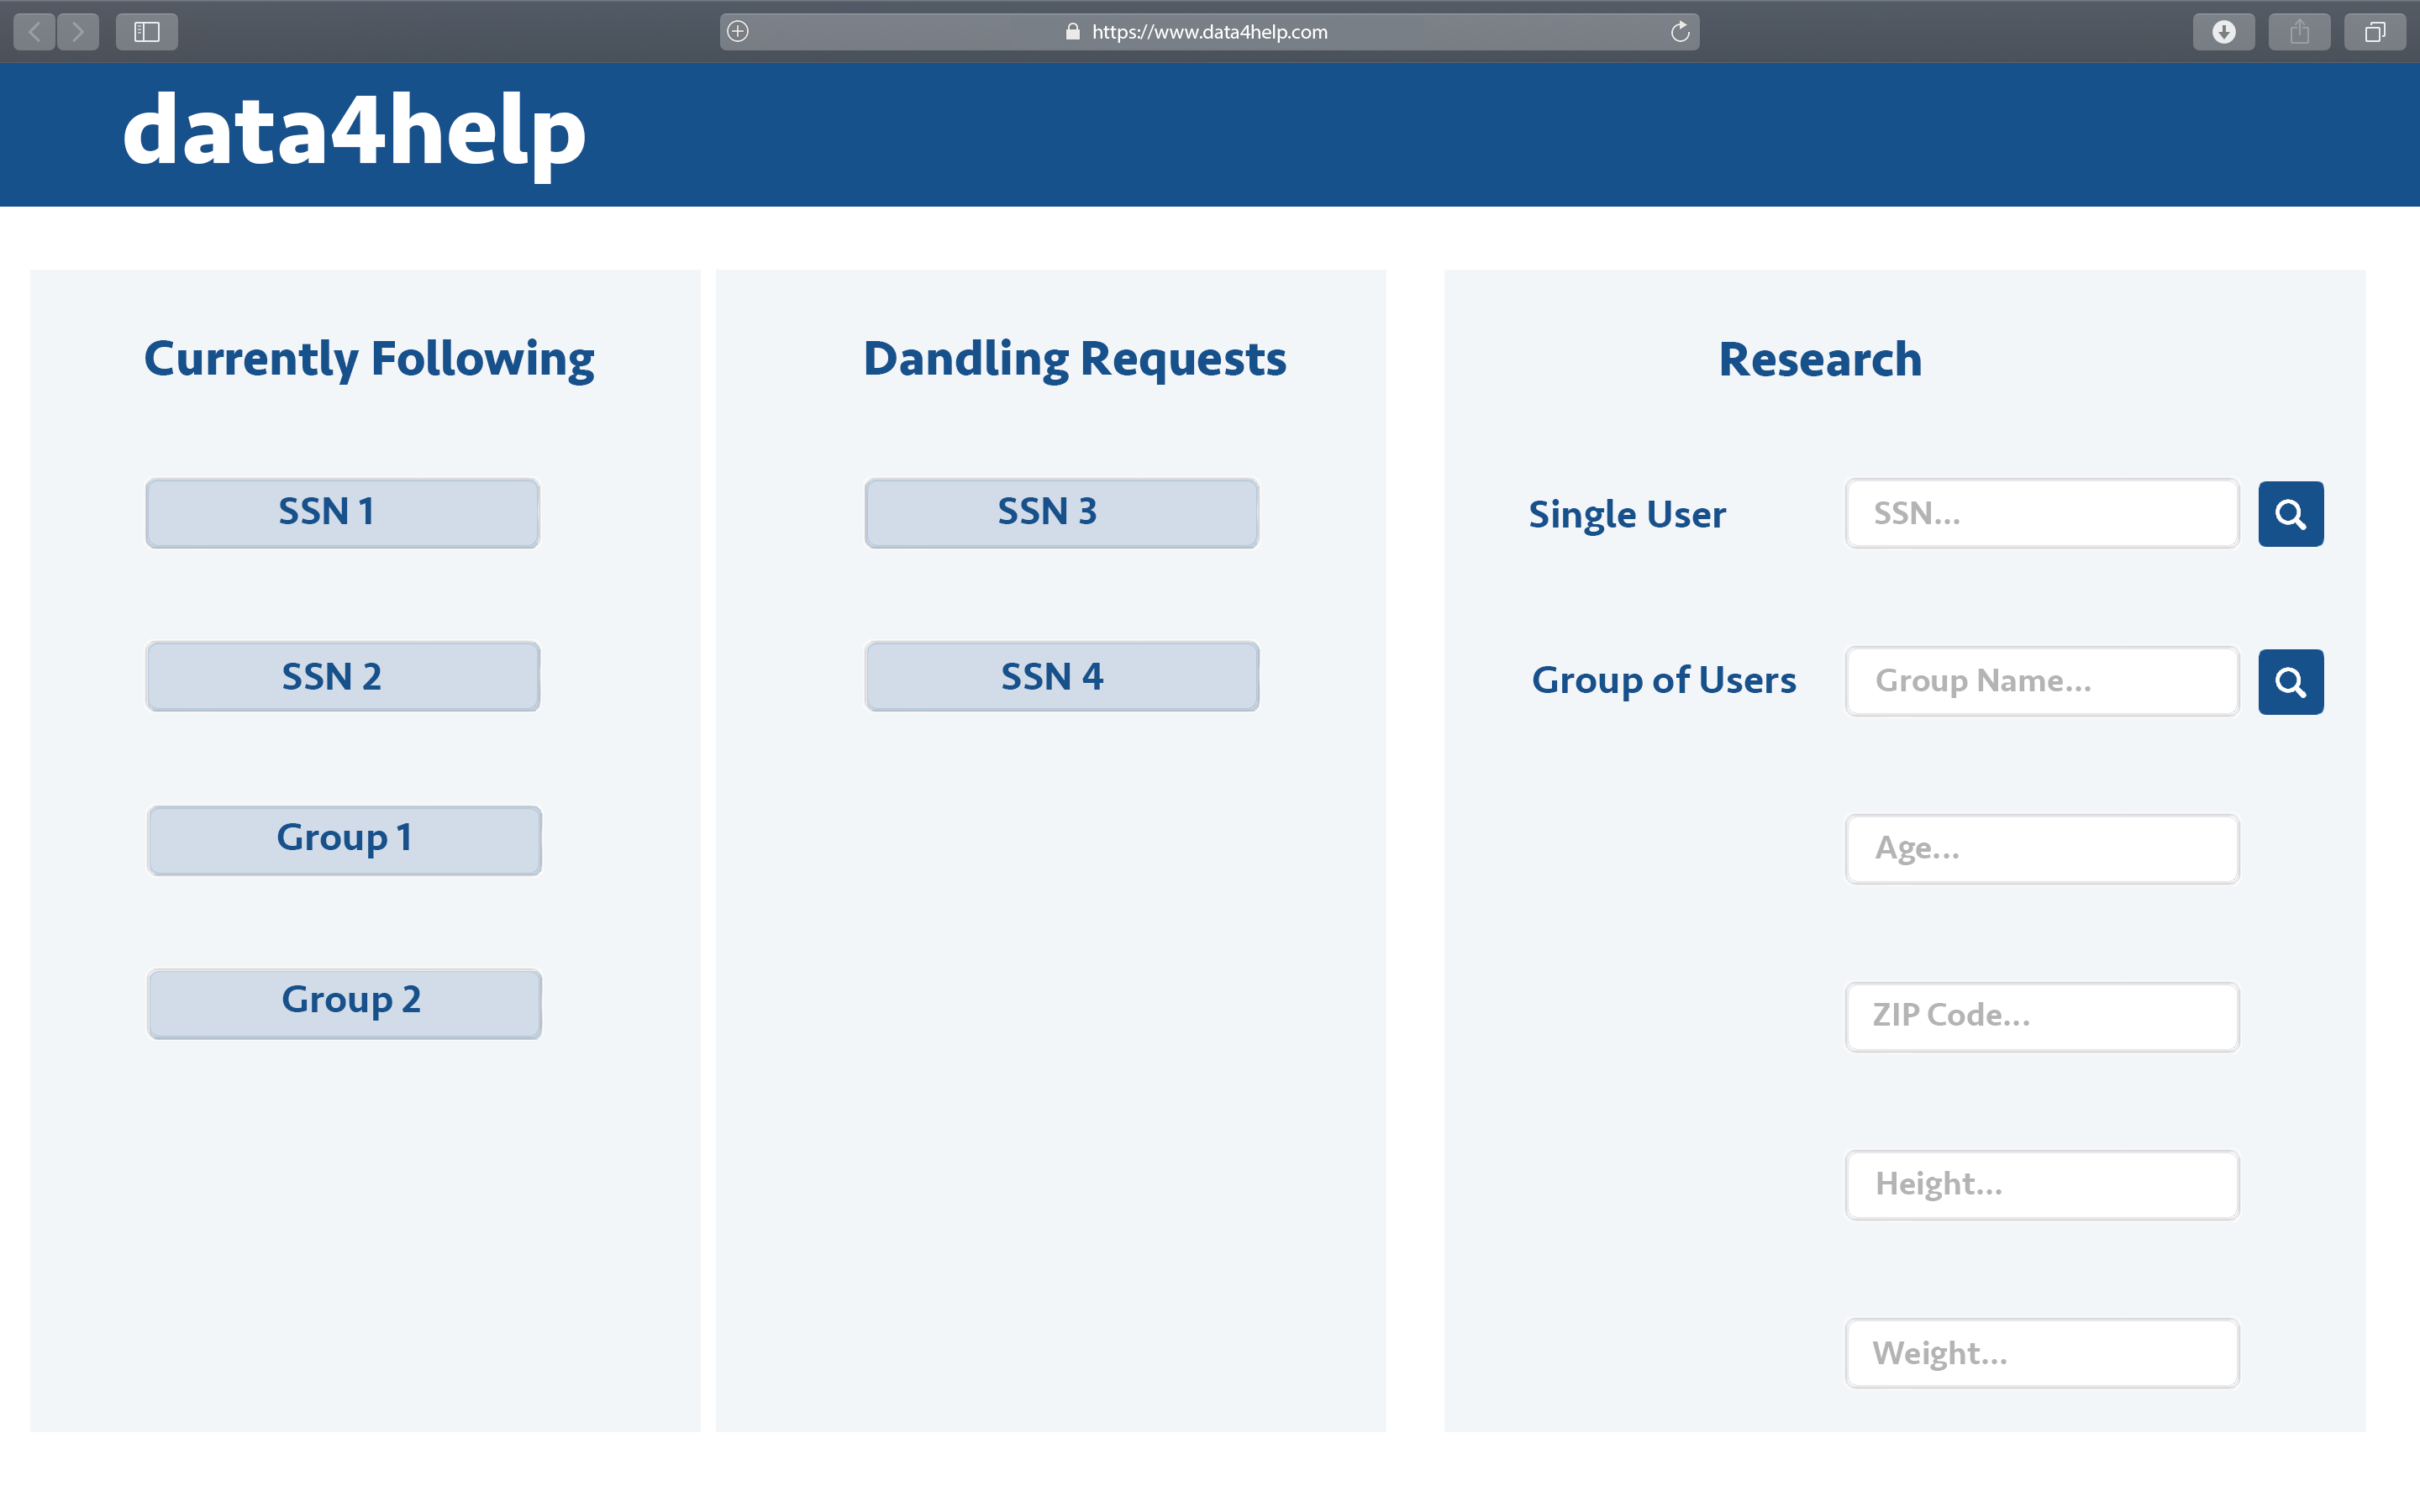
\includegraphics[width= \linewidth]{5companyhompage.png}
\end{figure}
\begin{figure}[h!]
\centering
    \textbf{Single user's data.}\par\medskip
	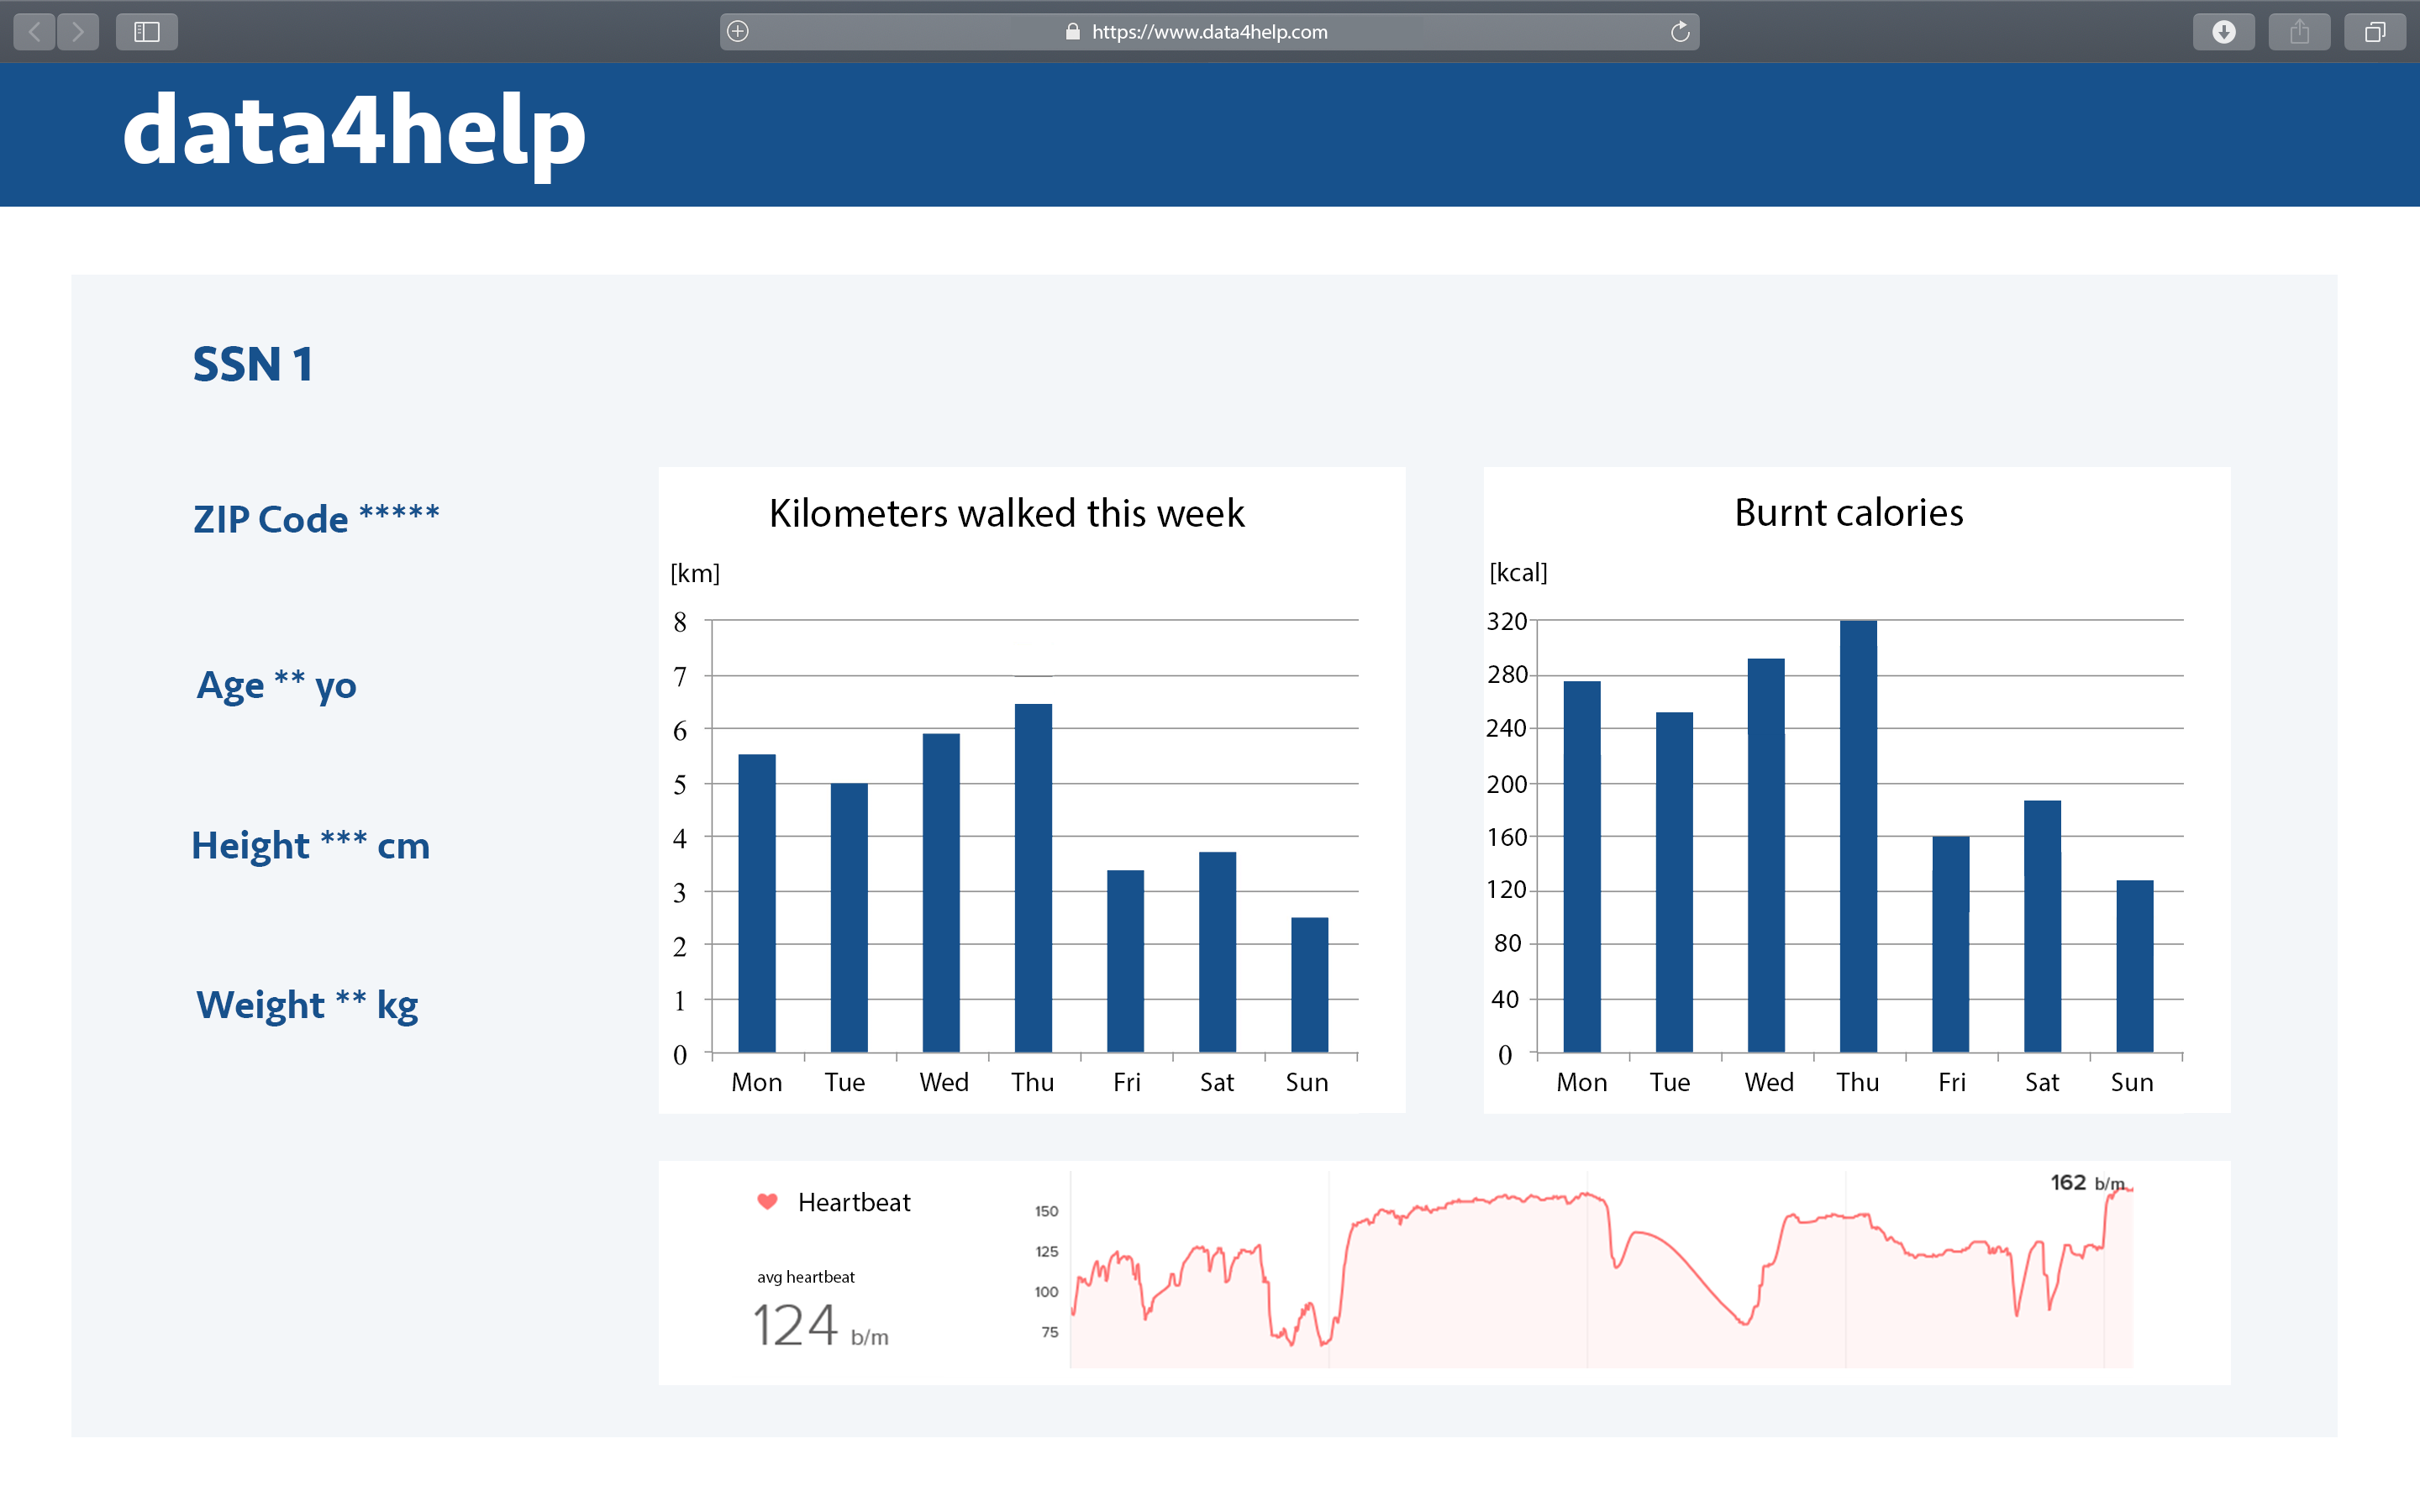
\includegraphics[width= \linewidth]{6userprofile.png}
\end{figure}\newpage
\begin{figure}[h!]
\centering
    \textbf{Group users' data.}\par\medskip
	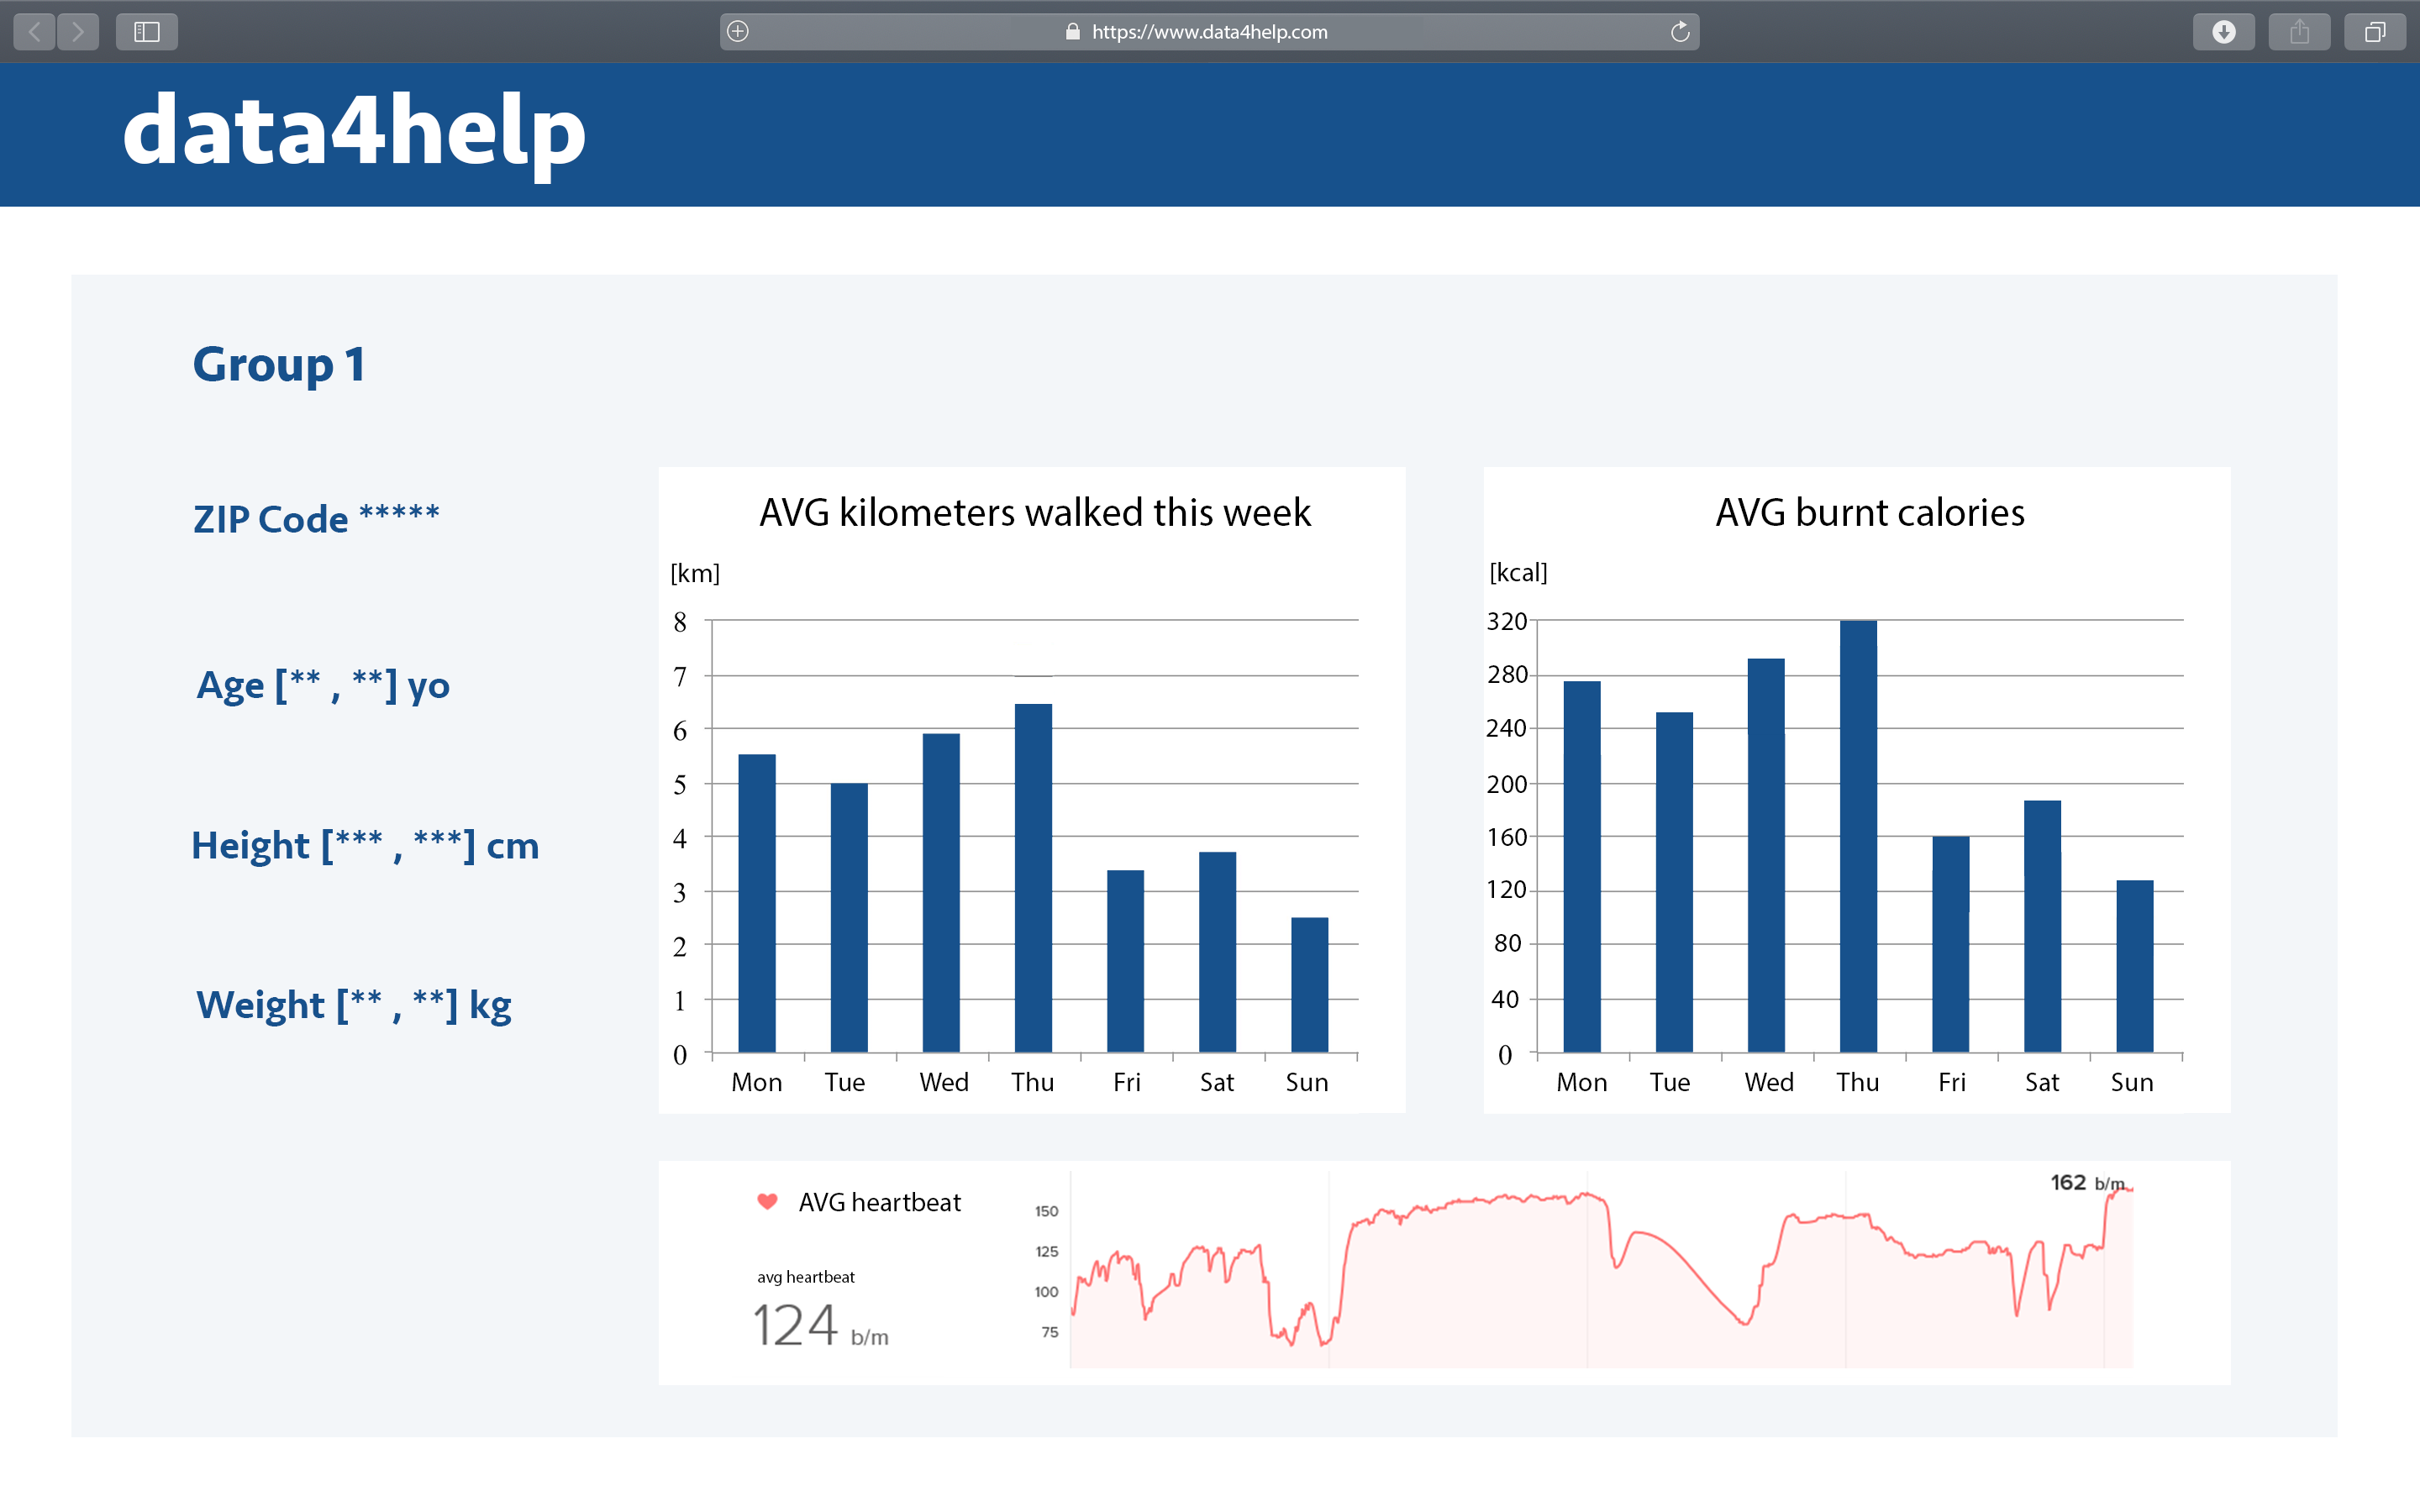
\includegraphics[width= \linewidth]{7groupprofile.png}
\end{figure}\newpage
\subsubsection{Hardware interfaces}
\begin{itemize}
	\item GPS
	\item Internet Connection(LTE)
	\item Photoplethysmography (PPG): integrated in the smart watch to monitor the heart rate of the user.
	\item Accelerometer: integrated in the smart watch and used to acquire data.
\end{itemize}
\subsubsection{Software interfaces}
\begin{itemize}
	\item Email Service: external interface used to forward the single user request from company to user and the other way around. 
	\item Ambulance Service: external interface with which AutomatedSOS will interact. 
\end{itemize}
\subsubsection{Communication interfaces}
The network-connected background app uses LTE to send data to TrackMe server. Companies access https://www.data4help.com through the HTTPS protocol. This must be guaranteed because of the sensible data that are present in the web site page.  
\subsection{Scenarios}
\subsubsection{Scenario 1}
Accenture wants to monitor the health status of its managers and decides to rely on Data4Help, thus signs up on Data4Help website.
Accenture's manager decided to try Data4Help only on one manager, Paolo, before starting with all the others. Paolo already has an Apple Watch, he signs up on Data4Help website.
In order to monitor Paolo's data, Accenture logs into the website and performs a request for data of a single user by inserting Paolo's SSN, that they know already.
Data4Help sends Paolo an email, notifying him that Accenture wants to see his data.
Paolo accepts Accenture's request by clicking on the corresponding link.
Once that Paolo accepted, Data4Help redirects Accenture on Paolo's profile page, and shows his main personal data: age, city, weight, height, kilometers walked during the current week, calories burnt during the current week and his average heartbeat during the day.
In the end Data4Help asks Accenture if is interested in being kept updated with Paolo's new data, Accenture answers yes.
\subsubsection{Scenario 2}
Allianz want to create a new insurance policy for people living in Milan, whose cost changes based on the lifestyle of the customer. In orded to make some statistical analisys Allianz relys on Data4Help.
Allianz subsrcibes on Data4Help website and performs a request for a group of users, searching for all the users living in Milan with age between 25 and 65 years old.
Data4Help performs the research and the outcome number is higher than 1000 users, thus data can be considered as anonymous and are shown to Allianz.
\subsubsection{Scenario 3}
San Raffaele hospital wants to create a new service in order to monitor its patients that previously had a stroke. They rely on AutomatedSOS. Each patient is given a smart watch and is subscribed to Data4Help website. Happens that Elena, one of the patients involved in this new service, has a stroke. In 3.7 seconds the hospital receives her current position due to an ambulance request.
\subsection{Functional requirements}
\subsubsection{[G1] Visitor can become User after providing credentials.}
\begin{itemize}
\item {[R1]} The system must allow a visitor to begin the registration process. During the process the system will ask him to provide credentials.
\item {[D6]} During the registration process the user inserts all the requested data.
\item {[D7]} The user has the physical characteristics that he inserted in the system.
\end{itemize}
\subsubsection{[G2] User can accept or reject the request of access to his data formulated by companies.}
\begin{itemize}
\item {[D1]} The user's email is already known by TrackMe.
\item {[R2]} Each time that an accepting or rejecting notification is sent to Data4Help, the system must mark a \emph{Pendent User} as not pendent anymore.
\item {[R3]} Each time that a user changes state from pendent to non-pendent, the corresponding single user request in the company list moves from dandling to accepted.
\end{itemize}
\subsubsection{[G3] If user's parameters are below specified thresholds, an ambulance is called within 5 seconds. [G3.1] Ambulance is required at current user's location.}
\begin{itemize}
\item {[R4]} The system must be able to monitor the user heart rate through hardware interfaces that are installed in the smart watch.
\item {[D4]} Smart watch in which the system-to-be is installed have: \emph{GPS, Accelerometer, LTE, Photoplethysmography}.
\item {[D5]} When the system shows the position of a user it means that the user is actually there.
\item {[D3]} At most 5 seconds are necessary to send user location and call an ambulance when parameters are below the threshold.
\end{itemize}
\subsubsection{[G4] Company can sign up as Company to Data4Help and AutomatedSOS.}
\begin{itemize}
\item {[R5]} The system must allow a company to begin the registration process. During the process the system will ask to provide credentials.
\item {[D2]} Only real companies can sing up as compaines.
\item {[R6]} At the end of the registration process, the system must provide to the company a password. The tuple $(VAT_number, password)$ is stored in the DB as unique.
\item {[D8]} Companies have a name and a vat number. VAT number is unique.
\end{itemize}
\subsubsection{[G5] Company can be recognized providing a password and vat number.}
\begin{itemize}
\item {[D8]} Companies have a name and a vat number. VAT number is unique.
\item {[R7]} The company can log in to the website by providing the combination of a name and a password that match its account.
\end{itemize}
\subsubsection{[G6] Company can formulate a request to see anonymized data of a group of users.}
\begin{itemize}
\item {[R8]} The system must allow the company to formulate a group of users request and fill it with drop down menu.
\item {[R9]} The system must allow the company to see its own request and their status(dandling, accepted or rejected).
\end{itemize}
\subsubsection{[G7] Company can formulate a request to see data of a specific user providing his SSN.}
\begin{itemize}
\item {[R10]} The system must allow the company to formulate a single user request and fill it with a valid SSN of a user.
\item {[R9]} The system must allow the company to see its own request and their status(dandling, accepted or rejected).
\end{itemize}
\subsubsection{[G8] Company can see anonymized data of a group of users.}
\begin{itemize}
\item{[R11]} The system must create a group if and only if more than 1000 user exists. 
\item {[R12]} The system must be able to anonymize data. The system must be able to access the DB where all the data are stored, perform researches based on the type of filter present in the group user request and once these information are retrieved fetch all the data that are related to a specific user(meaning all the information through which data can be related to a specific user).
\item {[R13]} The system must allow companies to see the data belonging to a group and for which exist the group request.
\end{itemize}
\subsubsection{[G9] Company can see data of a specific user providing his SSN.}
\begin{itemize}
\item {[D9]} Companies know the SSN of the user.
\item {[R14]} The system must allow companies to see data of a single user if the single user request exists and if the user approved that request.
\end{itemize}
\subsubsection{[G10] Company can subscribe to users’ new data.}
\begin{itemize}
\item {[R15]} The system must allow companies to see users' data as soon as they are produced.
\end{itemize}
\subsubsection{[G11] Data4Help can forward companies’ requests to users.}
\begin{itemize}
\item {[D1]} The user’s email is already known by TrackMe.
\item {[R9]} The system must allow the company to see its own request and their status(dandling, accepted or rejected).
\item {[R16]} The system must allow TrackMe to send an email to a user for which a company issue a single user request.
\end{itemize}
\subsubsection{[G12] A user of Data4Help becomes automatically a user of AutomateSOS if he is older than Age}
\begin{itemize}
\item {[R17]} Data4Help allow AutomatedSOS to see data of a user.
\item {[R18]} If a user insert as age a value grater or equal than \emph{Age} the system must automatically enroll this user to AutomatedSOS.
\item {[R19]} If the age inserted by the user + the current data $>=$ than \emph{Age} the system must automatically enroll this user to AutomatedSOS. 
\end{itemize}\newpage
\subsubsection{Use case diagram}

\begin{figure}[h!]
\centering
    \textbf{}\par\medskip
	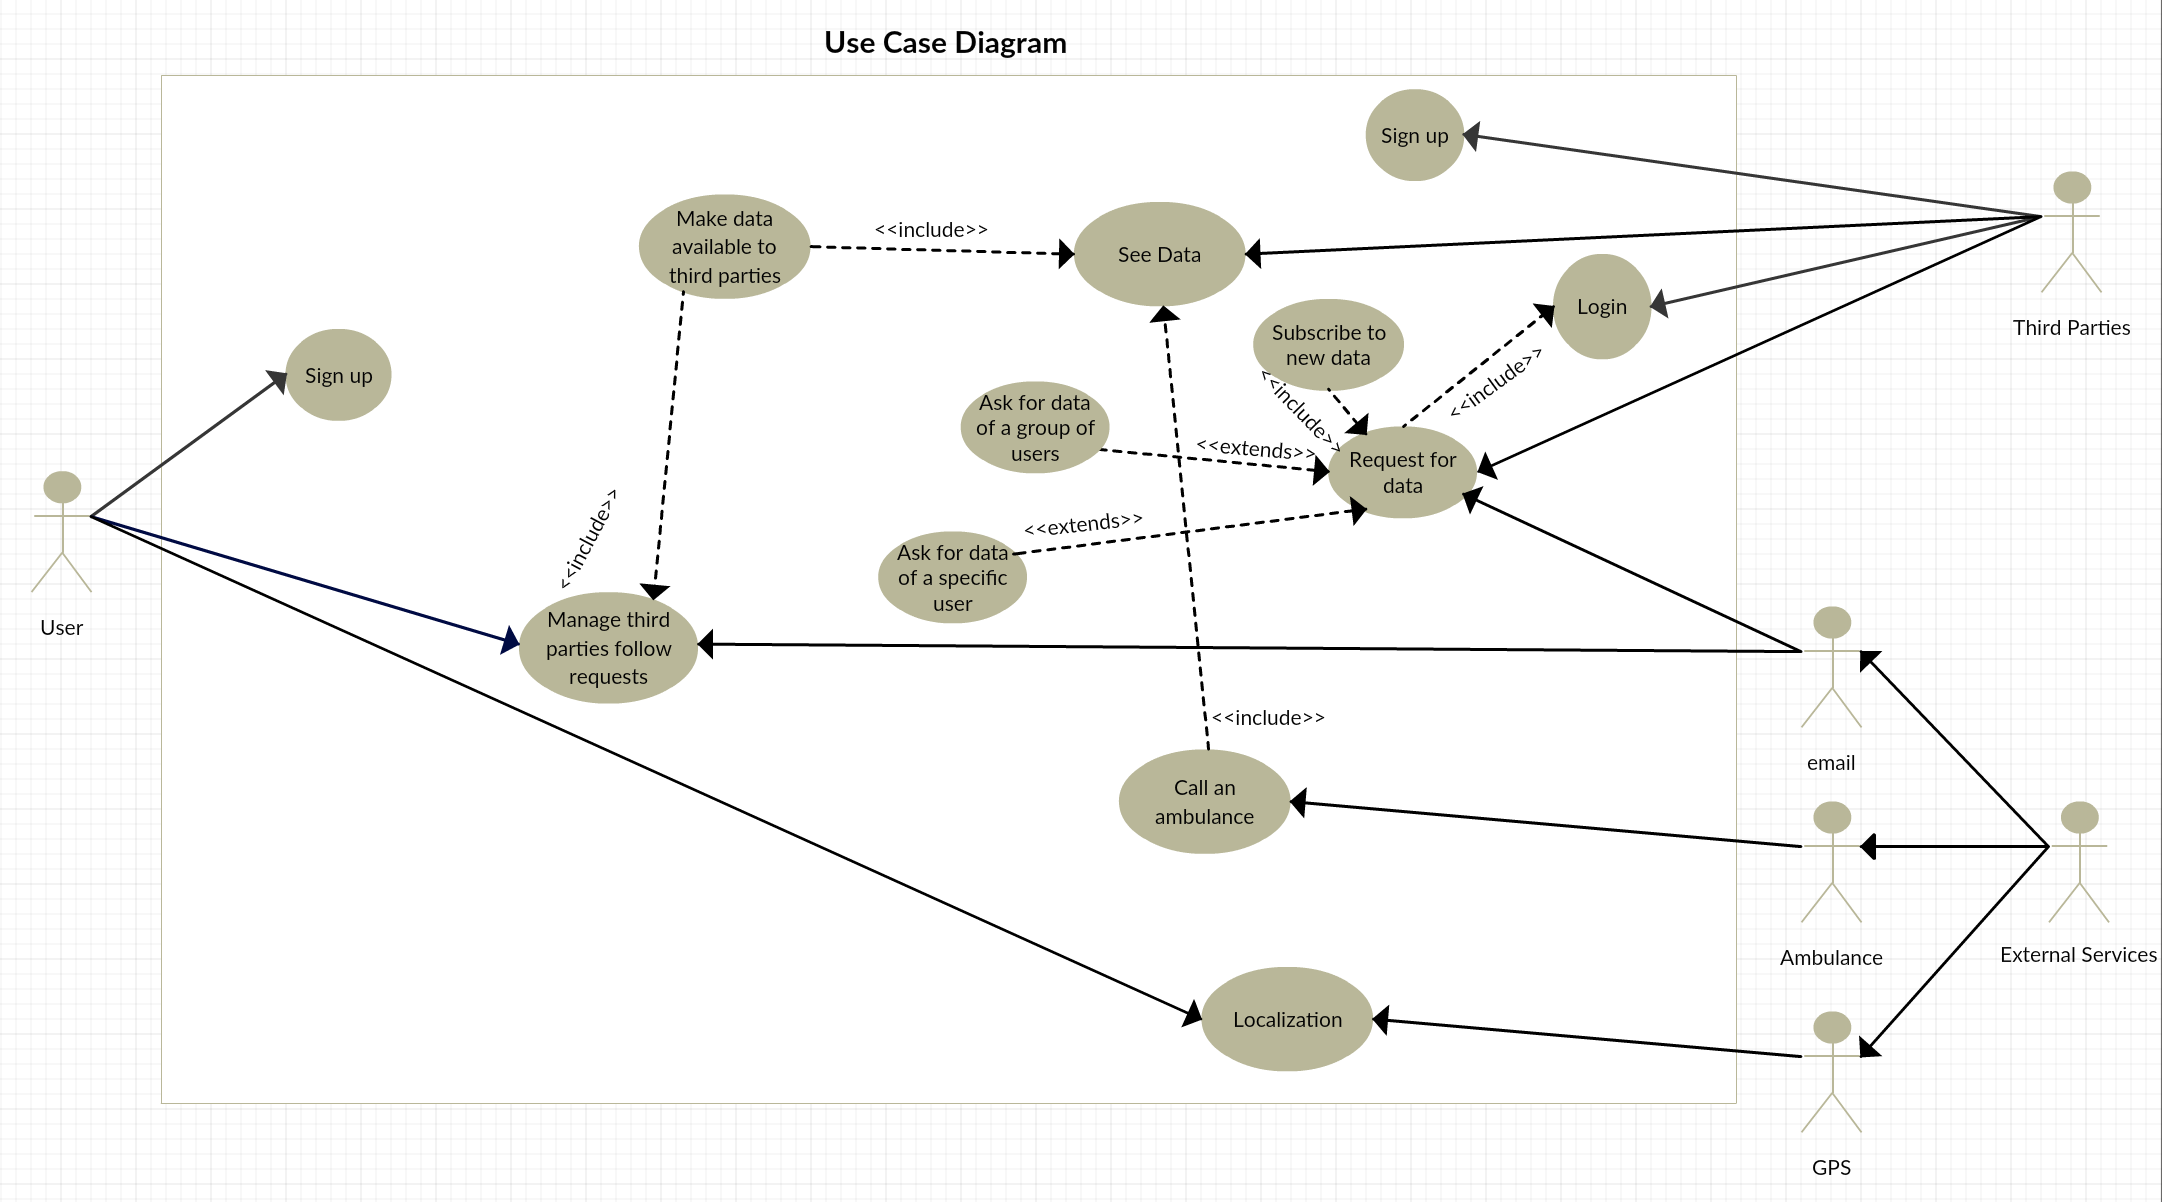
\includegraphics[width= \linewidth]{usecase.png}
\end{figure}
\begin{center}
    \begin{tabular}{ | l | p{10cm} |}
    \hline
    Name & Visitor sing up.\\ \hline
    Actors & User\\ \hline
   	Goals & {[G1]}\\ \hline
    Input Conditions & There are no entry conditions.\\ \hline
    Event Flow & \begin{enumerate}
    	\item The user on the web home page clicks on the sign in button to start the registration process.
    	\item The user insert his Google account or Apple account.
    	\item The user fills all the mandatory fills.
		\item The user clicks on the confirm button.
		\item The system saves the data.
    \end{enumerate} \\ \hline
    Output Conditions & The user successfully ends the registration process. From now on he can use Data4Help and AutomatedSOS(if age is greater or equal than \emph{Age}). \\ \hline
    Exceptions & \begin{enumerate}
    	\item The user is already registered.
		\item The user inserts no valid information in one or more mandatory fills.
		\item The user chooses a Google account or Apple account that is already used.
	\end{enumerate}
All the exceptions are handled notifying the issues to the user and taking back the event flow to point 2.
    \\ \hline
    \end{tabular}
\end{center}

\begin{center}
    \begin{tabular}{ | l | p{10cm} |}
    \hline
    Name & User accept or reject third party requests.\\ \hline
    Actors & User\\ \hline
   	Goals & {[G2]}\\ \hline
    Input Conditions & The user receives a request of following.\\ \hline
    Event Flow & \begin{enumerate}
    	\item The user checks his email and open the following request.
		\item The user clicks the link present in the email.
		\item The user is redirected in the web page where I can accept or reject the request by clicking on one of the two button.
    \end{enumerate} \\ \hline
    Output Conditions & The user is notified to have actually accepted/reject the request. The company that issued that request is notified that a request has been accepted/rejected. The request is moved from dandling to accepted/rejected. If the user was \emph{pendent} just for this request, it is marked as \emph{not pendent} anymore. \\ \hline
    Exceptions & -\\ \hline
    \end{tabular}
\end{center}
\begin{center}
    \begin{tabular}{ | l | p{10cm} |}
    \hline
    Name & Third part sign up.\\ \hline
    Actors & Third part\\ \hline
   	Goals & {[G4]}\\ \hline
    Input Conditions & There are no entry conditions.\\ \hline
    Event Flow & \begin{enumerate}
    	\item The third part on the home page clicks on the sign in button to start the registration process.
		\item The third part fills all the mandatory fills.
		\item The third part clicks on the confirm button.
		\item The system saves the data.
    \end{enumerate} \\ \hline
    Output Conditions & The third part successfully ends the registration process. From now on it can log into the application, providing his credentials and start using Data4Help and AutomatedSOS.  \\ \hline
    Exceptions & \begin{enumerate}
    \item The third part is already registered.
	\item The third part inserts no valid information in one or more mandatory fills.
	\item The third part chooses a vat number that has already been taken. 
\end{enumerate} All the exceptions are handled notifying the issues to the third part and taking back the event flow to point 2.  \\ \hline
    \end{tabular}
\end{center}

\begin{center}
    \begin{tabular}{ | l | p{10cm} |}
    \hline
    Name & Third part login.\\ \hline
    Actors & Third part\\ \hline
   	Goals & {[G5]}\\ \hline
    Input Conditions & There third part is already in the homepage.\\ \hline
    Event Flow & \begin{enumerate}
    	\item The third part inserts its credentials in.
		\item The third part clicks on the login button in order to access.
		\item The system redirects the third part to his profile.
    \end{enumerate} \\ \hline
    Output Conditions & The third part his successfully redirects to his profile.  \\ \hline
    Exceptions & \begin{enumerate}
   \item The third part insert a not vat number.
	\item The third part insert a not valid password.
\end{enumerate} All the exceptions are handled notifying the issues to the user and taking back the event flow to point 1.    \\ \hline
    \end{tabular}
\end{center}

\begin{center}
    \begin{tabular}{ | l | p{10cm} |}
    \hline
    Name & Third part formulate a request to access anonymized data of a group of users.\\ \hline
    Actors & Third part\\ \hline
   	Goals & {[G6]}\\ \hline
    Input Conditions & The third part is already logged in into the system.\\ \hline
    Event Flow & \begin{enumerate}
    	\item The third part clicks on the \emph{group request}.
    	\item The request is filled using drop-down menu. Each drop-down menu is linked to a type of filter. By selecting a filter the company is able to better specify the composition of the group it is interested in.
		\item The request is sent to TrackMe's servers by clicking on \emph{send} button. 
    \end{enumerate} \\ \hline
    Output Conditions & The request is sent to TrackMe and a message for the correct sending of the request is presented to the company. \\ \hline
    Exceptions & -   \\ \hline
    \end{tabular}
\end{center}

\begin{center}
    \begin{tabular}{ | l | p{10cm} |}
    \hline
    Name & Third part formulate a request to access data of a specific user through is SSN. \\ \hline
    Actors & Third part\\ \hline
   	Goals & {[G7]}\\ \hline
    Input Conditions & The third part is already logged in into the system.\\ \hline
    Event Flow & \begin{enumerate}
    	\item The third part clicks on the \emph{single user request}.
    	\item The request is filled with the user's SSN.
    	\item The request is sent to TrackMe by clicking on \emph{send} button. 
    \end{enumerate} \\ \hline
    Output Conditions & The request is sent to TrackMe's servers and a message for the correct sending of the request is presented to the company.  \\ \hline
    Exceptions & -    \\ \hline
    \end{tabular}
\end{center}

\begin{center}
    \begin{tabular}{ | l | p{10cm} |}
    \hline
    Name & Third part can access anonymized data of a group of users.\\ \hline
    Actors & Third part\\ \hline
   	Goals & {[G8]}\\ \hline
    Input Conditions & There third part is already logged into the system and a group request for this group exists.\\ \hline
    Event Flow & \begin{enumerate}
    	\item The third part accesses the approved group requests section.
		\item The third part selects an approved group request.
		\item The system redirects the third part to the request result.
    \end{enumerate} \\ \hline
    Output Conditions & The data requested by the third part are shown.  \\ \hline
    Exceptions & \begin{enumerate}
  		\item The data requested aren't anonymous since the outcome of the request concerns less than 1000 users.
\end{enumerate} All the exceptions are handled notifying the issues to the third part and taking back the event flow to point 1.    \\ \hline
    \end{tabular}
\end{center}

\begin{center}
    \begin{tabular}{ | l | p{10cm} |}
    \hline
    Name & Third part can access data of a specific user through his SSN.\\ \hline
    Actors & Third part\\ \hline
   	Goals & {[G9]}\\ \hline
    Input Conditions & There third part is already logged into the system.\\ \hline
    Event Flow & \begin{enumerate}
    	\item The third part accesses the approved single user requests section.
    	\item The third part selects an approved single user request. 
    	\item The system redirects the third part to the request result.
    \end{enumerate} \\ \hline
    Output Conditions & The data requested by the third part are shown.  \\ \hline
    Exceptions & \begin{enumerate}
   \item The user didn't approve the request.
\end{enumerate} All the exceptions are handled notifying the issues to the third part and taking back the event flow to point 1.    \\ \hline
    \end{tabular}
\end{center}

\begin{center}
    \begin{tabular}{ | l | p{10cm} |}
    \hline
    Name & Data4Help can forward third parties requests to users. \\ \hline
    Actors & Data4Help\\ \hline
   	Goals & {[G11]}\\ \hline
    Input Conditions & Third part has requested data of a single user.\\ \hline
    Event Flow & \begin{enumerate}
    	\item Data4Help forwards the request of being observed by a specific company to the user using the external email service.
    	\item Data4Help marks the user as \emph{pendent user}.
    \end{enumerate} \\ \hline
    Output Conditions & The request of being followed by a company is sent to the user. \\ \hline
    Exceptions & -    \\ \hline
    \end{tabular}
\end{center}


\begin{center}
    \begin{tabular}{ | l | p{10cm} |}
    \hline
    Name & A User of Data4Help becames automatically a user of AutomateSOS. \\ \hline
    Actors & Data4Help\\ \hline
   	Goals & {[G12]}\\ \hline
    Input Conditions & User sign up.\\ \hline
    Event Flow & \begin{enumerate}
    	\item Data4Help checks the age of the user + current date.
    	\item Data4Help subscribes the user to AutomatedSOS.
    \end{enumerate} \\ \hline
    Output Conditions & User is notified than he has been subscribed to AutomateSOS, through an email. \\ \hline
    Exceptions & \begin{enumerate}
    	\item User's age + current date is less than \emph{Age}.
\end{enumerate}  The user is not enrolled in AutomatedSOS.   \\ \hline
    \end{tabular}
\end{center}\newpage

\subsubsection{Sequence diagram}

\begin{figure}[h!]
\centering
    \textbf{Company formulate single user request.}\par\medskip
	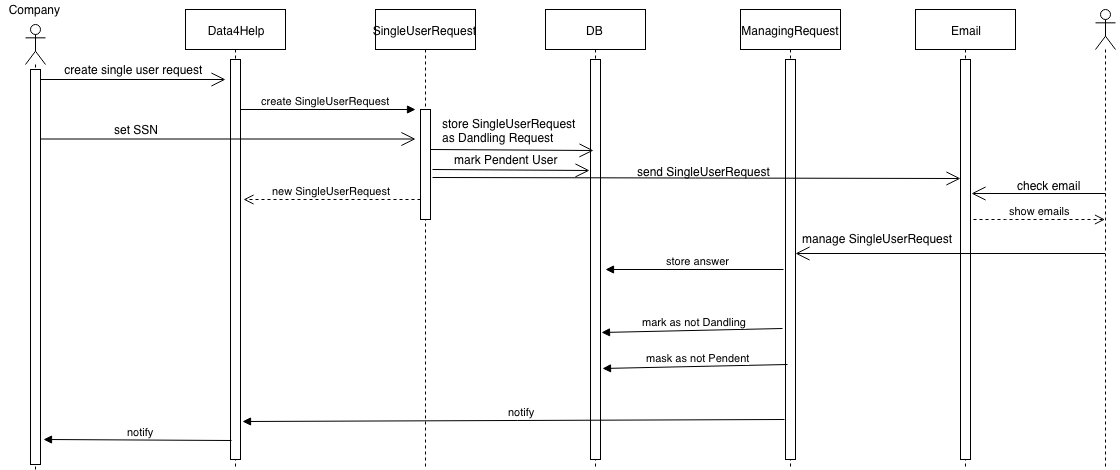
\includegraphics[width= \linewidth]{singlerequest.png}
\end{figure}\newpage
\begin{figure}[h!]
\centering
    \textbf{Company formulate group user request.}\par\medskip
	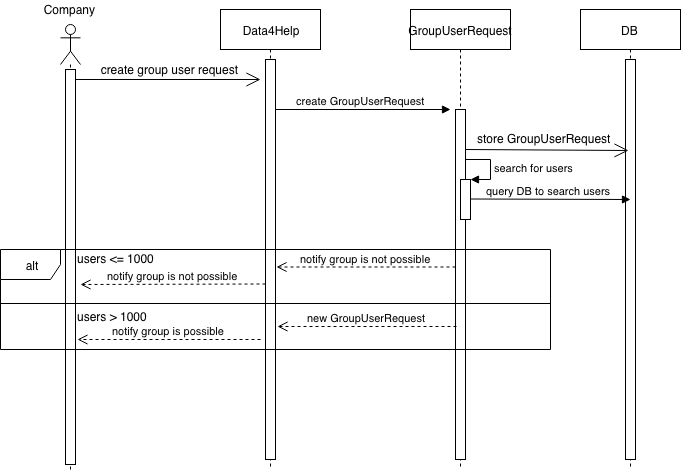
\includegraphics[width= \linewidth]{grouprequest.png}
\end{figure}\newpage
\begin{figure}[h!]
\centering
    \textbf{AutomatedSOS calls an ambulance.}\par\medskip
	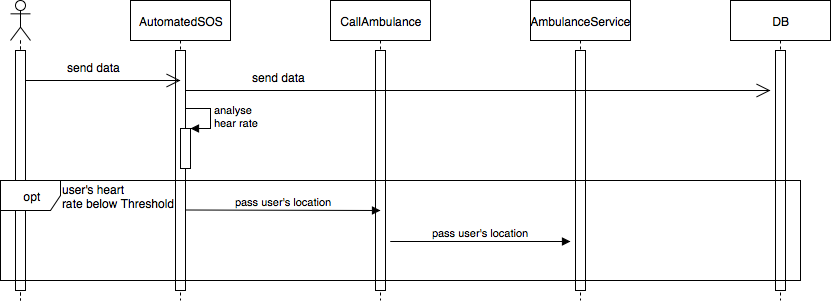
\includegraphics[width= \linewidth]{callambulance.png}
\end{figure}\newpage
\subsection{Performance requirements}
When hear rate of user is below the \emph{Threshold}, AutomatedSOS calls an ambulance to the current user's position within 5 seconds. This is the most important \emph{non-functional} constraint of the all system-to-be. Users will rely on the application in order to be sure, during their everyday activities, that they will be safe in case of dangerous heart dysfunction. During the test phase, this requirement must be tested with the high priority. 
\subsection{Design constraints}
\subsubsection{Standard compliance}
\begin{itemize}
\item The app requires permission to access user current position.
\item Personal data processing observes GDPR
\item Users' data are stored in TrackMe's servers.
\item Website access is guaranteed to be safe by using HTTPS
\end{itemize}
\subsubsection{Hardware limitation}
In order to work properly the system-to-be needs to be installed in a smart watch that has at least these hardware:
\begin{itemize}
\item a wearable device with watchOS or wearOS
\item GPS
\item Photoplethysmography (PPG)
\item Accelerometer
\item LTE
\end{itemize}
\subsubsection{Other constraints}
\begin{itemize}
\item Regulatory policies
\item Usage is possible only for users with a Google or iOS account
\item The smart watch must be logged in a Google or iOS account
\end{itemize}
\subsection{Software system attributes}
\subsubsection{Reliability}
The application must be available 24/7. Since AutomatedSOS is built on top of Data4Help, no concession is tolerated. Obviously it is not feasible to reach a 100\% of availability, but a 99.999\% of availability is required. This constraints will result in a high cost of architecture design and will automatically bring to replication of core systems of the system-to-be. If an availability of 99.999\% will result not feasible this must be indicated to the management and clearly stated in the legal contract of this product.
\subsubsection{Security}
Due to the sensitive nature of these data, security is an important issue. Web access will use HTTPS protocol in order to limit the probability of malicious attacks. Data will be store in DB using all the required techniques that helps to improve security of data. In order to accomplish the industry's standards, \emph{ISO-14971} should be consulted.
\subsubsection{Maintainability}
Code is structured in such a way that possible future modification and functionality addition will be easy to implement, e.g. Track4Run, a service to track athletes participating in a run.
\subsubsection{Compatibility}
The website is compatible with Google Chrome, Safari and Firefox. \\
The background app is compatible only with smart watch running on Watch OS and Wear OS.
\newpage
\section{Formal Analysis Using Alloy}
\subsection{Alloy model}
open util/integer \\ 
open util/boolean \\
\\
 sig User \{  \\
 age: one Int, \\ 
 height: one Int, \\ 
 weight: one Int, \\
 ssn: one String, \\ 
 residence: one Int, --This is the user's CAP \\ 
 datas: Data, \\
 requests: set Request,  \\
 \}   \{ \\
 age $\geq$ 0 and \\ 
 height $\geq$ 0 and  \\ 
 weight $\geq$ 0 \\ 
 \} \\
 \\
sig Group \{\\
users: set User\\
\} \{ \\users $\geq$ 1001\\ \}\\
\\
sig Data \{\\
heartrate: one Int,\\
calories: one Int,\\
km: one Int,\\
locations: Location\\
\} \{\\
heartrate $\geq$ 0 and\\
calories $\geq$ 0 and\\
km $\geq$ 0\\
\}\\
\\
sig Location\{\\
cordX: one Int,\\
cordY: one Int\\
\} \{\\
cordX $\geq$ 0 and\\
cordY $\geq$ 0\\
\}\\
\\
sig Company\{\\
vat: one String,\\
name: one String,\\
password: one String,\\
requests: set Request \\
\}\\
\\
abstract sig Request\{\\
vatCompany: one String,\\
approve: one Bool\\
\}\\
\\
sig SingleUserRequest extends Request\{\\
ssn: one String\\
\}\\
\\
sig GroupUserRequest extends Request\{\\
groupname: one String,\\
filterbyresidence: one Int,\\
filterbyagelower: one Int,\\
filterbyagehigher: one Int,\\
filterbyheightlower: one Int,\\
filterbyheighthigher: one Int,\\
filterbyweightlower: one Int,\\
filterbyweighthigher: one Int\\
\}\{\\
filterbyresidence $\geq$ 0 and\\
filterbyagelower $\geq$ 0 and\\
filterbyagehigher $\geq$ 0 and\\
filterbyheightlower $\geq$ 0 and\\
filterbyheighthigher $\geq$ 0 and\\
filterbyweightlower $\geq$ 0 and\\
filterbyweighthigher $\geq$ 0 and\\
(filterbyagelower $\geq$ filterbyagehigher) and\\
(filterbyheightlower $\geq$ filterbyheighthigher) and\\
(filterbyweightlower $\geq$ filterbyweighthigher)\\
\}\\
\\
-- a signle request cannot exists on its own, or belong to more than one company\\
\\
fact SingleRequestCompanyconnection \{\\
all r:SingleUserRequest \textbar \space all c:Company \textbar \space (r in c.requests implies r.vatCompany = c.vat) and (r.vatCompany = c.vat implies r in c.requests)\\
\}\\
\\
fact SingleRequestUserconnection \{\\
all r:SingleUserRequest \textbar \space all u:User \textbar \space (r in u.requests implies u.ssn = r.ssn) and (r.ssn = u.ssn implies r in u.requests)\\
\}\\
\\
-- a group request cannot exists on its own, or belong to more than one company\\
\\
fact GroupRequestCompanyconnection \{\\
all r:GroupUserRequest \textbar \space all c:Company \textbar \space (r in c.requests implies r.vatCompany = c.vat) and (r.vatCompany = c.vat implies r in c.requests)\\
\}\\
\\
fact GroupRequestUserconnection \{\\
all g:GroupUserRequest \textbar \space all u:User \textbar \space (((g.filterbyagelower $\leq$ u.age and u.age $\leq$ g.filterbyagehigher) and\\ (g.filterbyheightlower $\leq$ u.height and u.height $\leq$ g.filterbyheighthigher) and\\ (g.filterbyweightlower $\leq$ u.weight and u.weight $\leq$ g.filterbyweighthigher) and\\ (g.filterbyresidence=u.residence))implies(g in u.requests))\\
\}\\
\\
-- vat is unique\\
\\
fact vatUnique\{\\
no disjoint c1,c2 : Company \textbar \space c1.vat = c2.vat\\
\}\\
\\
-- ssn is unique\\
\\
fact ssnUnique\{\\
no disjoint u1,u2 : User \textbar \space u1.ssn = u2.ssn\\
\}\\
\\
pred show ()\{\\
(some u:User \textbar \space u.requests $\geq$ 2 and u.ssn = "1234") and\\
(some u:User \textbar \space u.requests $\geq$ 2 and u.ssn = "5678") and\\
(some c:Company \textbar \space c.requests $\geq$ 1 and c.vat ="5043670") and \\
(one s:SingleUserRequest \textbar \space s.ssn = "1234" and s.vatCompany = "5043670") and\\
(one s:SingleUserRequest \textbar \space s.ssn = "5678" and s.vatCompany = "5043670") and\\
(one g:GroupUserRequest \textbar \space g.vatCompany = "4563729" and g.groupname = "nordMilano")\\
\}\\
run show\\
\newpage
\subsection{World generated}
\begin{figure}[h!]
	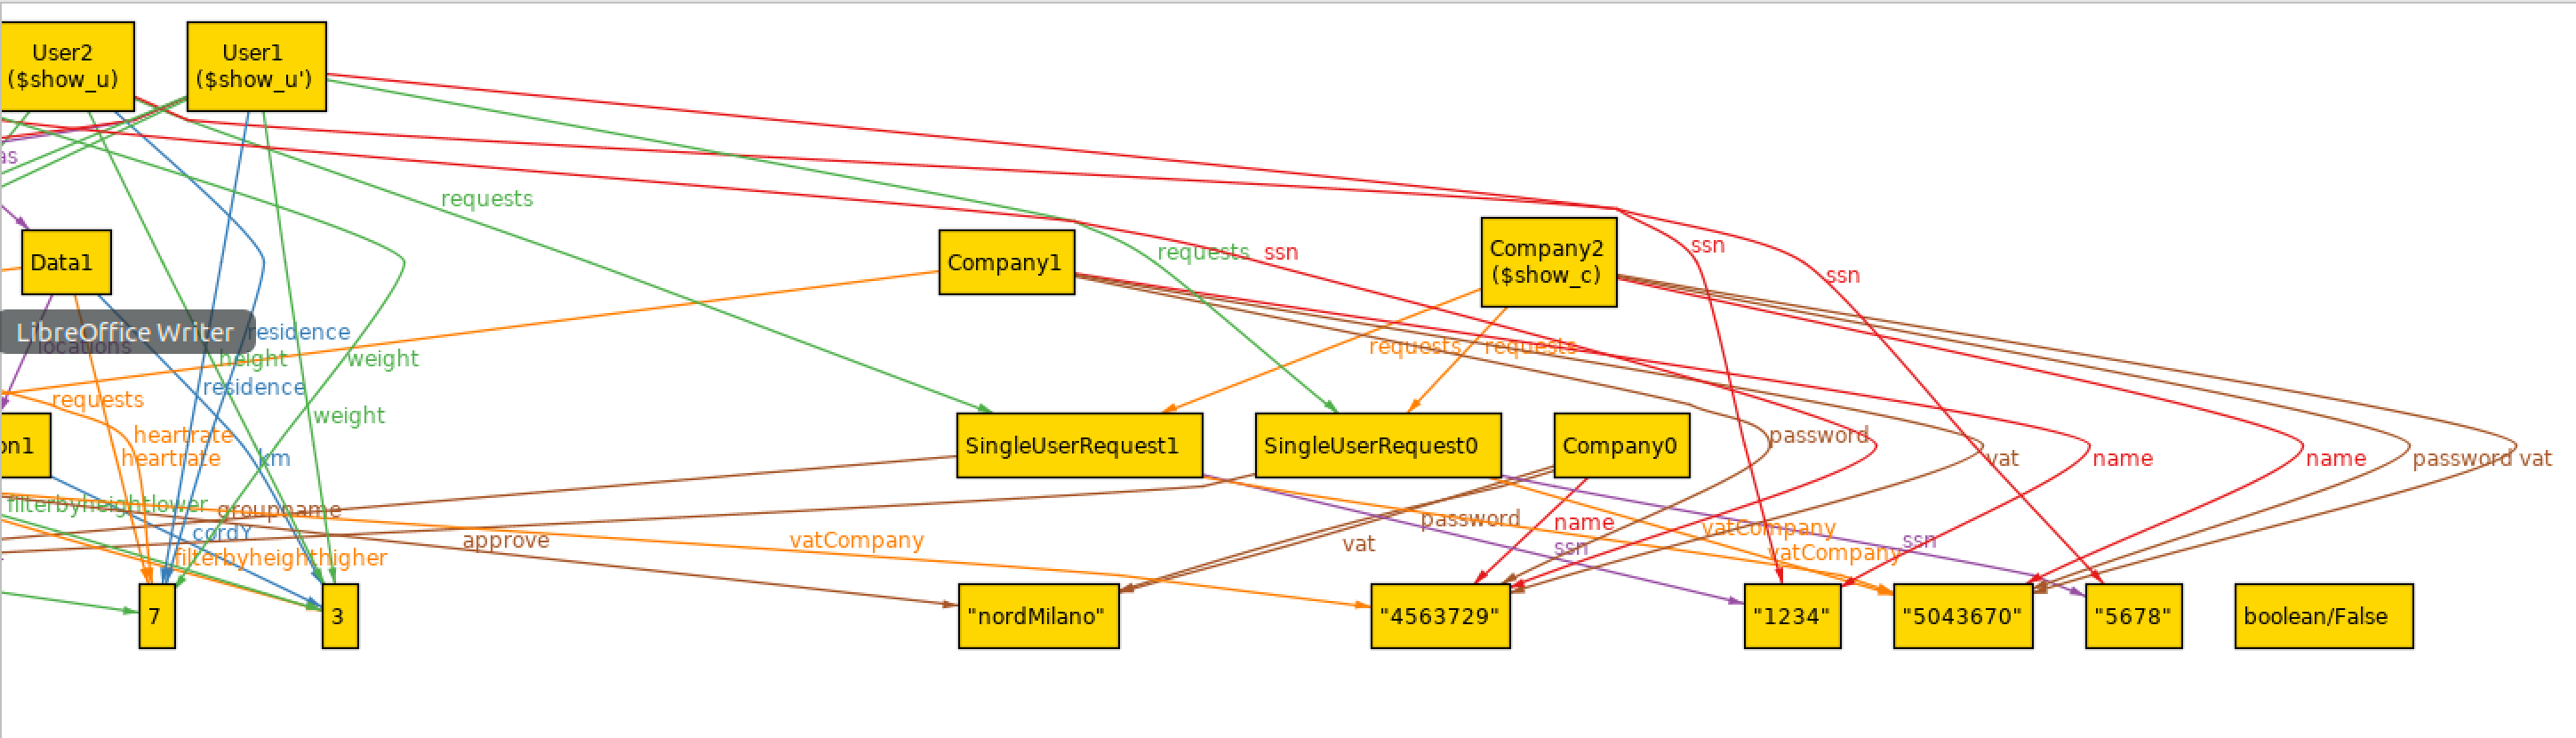
\includegraphics[width= \linewidth]{world1.png}
	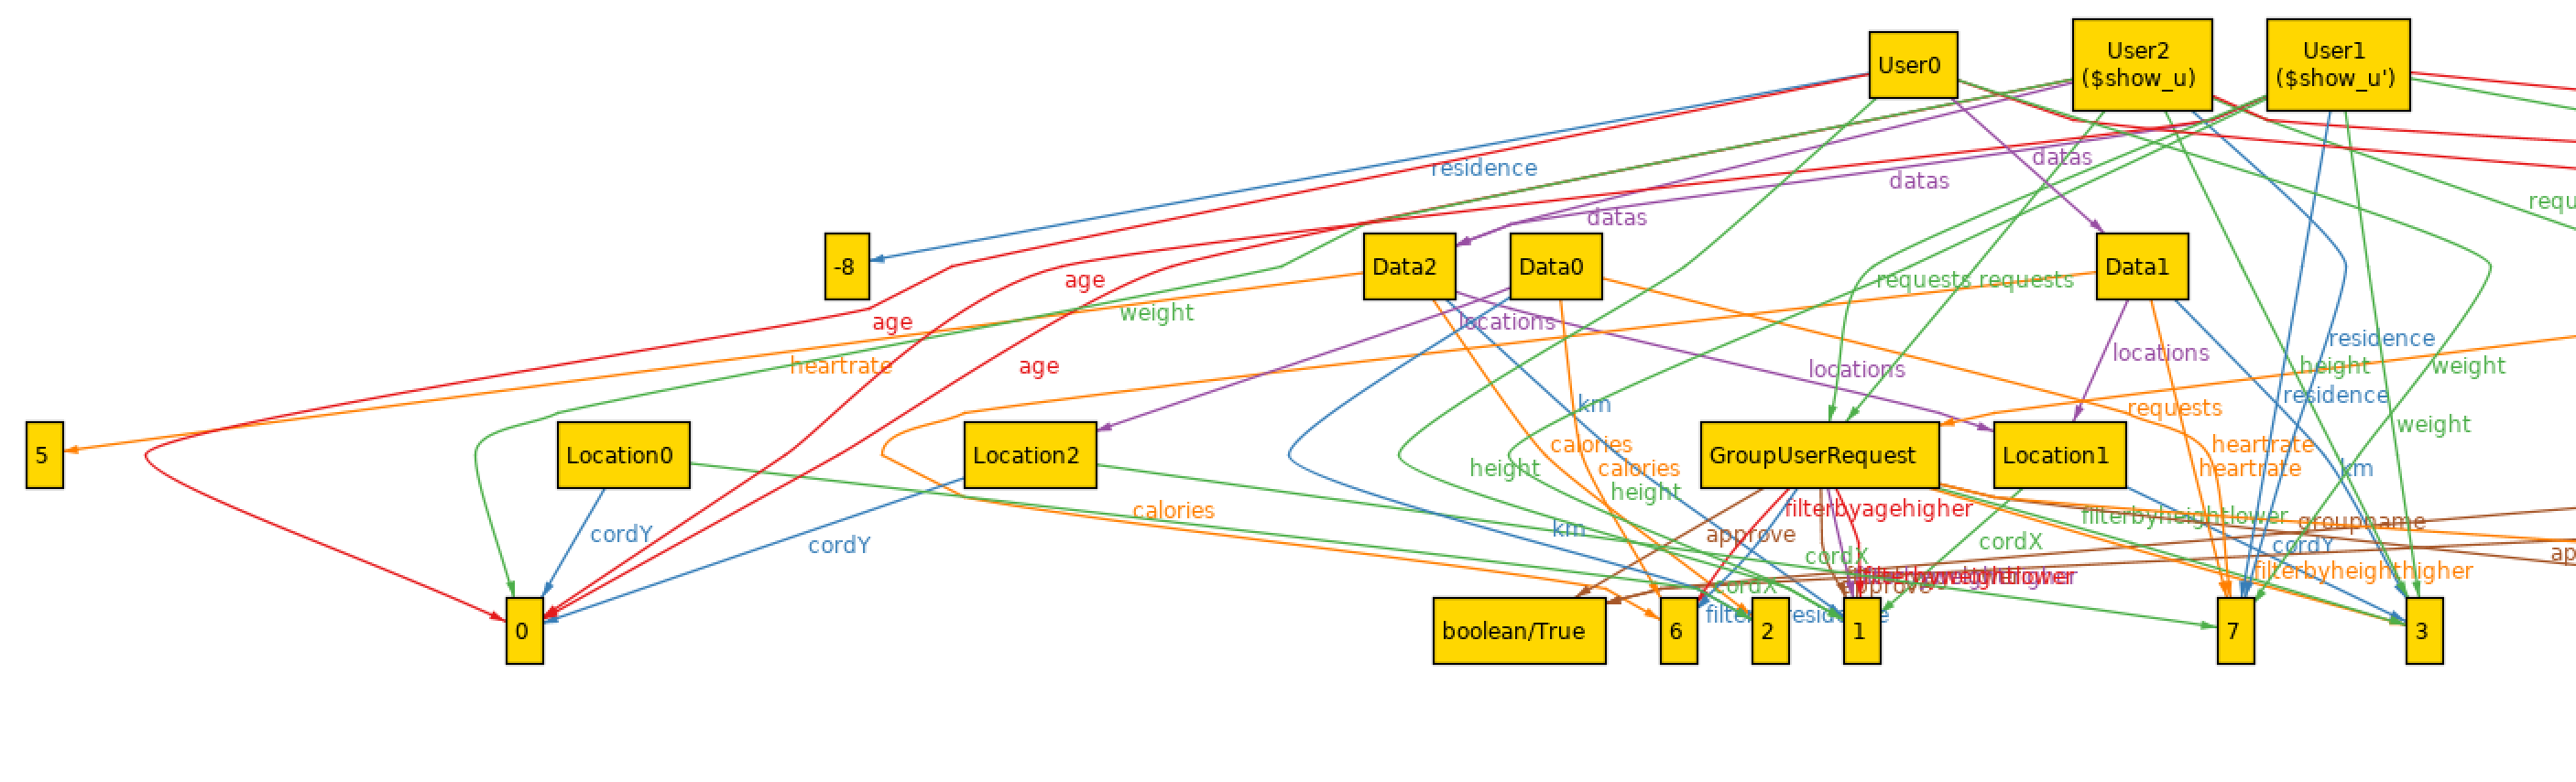
\includegraphics[width= \linewidth]{world2.png}
\end{figure}
\newpage
\subsection{Alloy results}
As we can see the model was able to find a world that satisfies all the facts. \\
The main point we wanted to highlight was the fact that our requests must be issued by a company and must be related to some user. \\
With our Alloy model we did that.
\newpage
\section{Effort Spent}
\subsection{Dalle Rive Fabio}
\begin{center}
    \begin{tabular}{ | l | r |}
    \hline
    \textbf{Task Description} & \textbf{Hours} \\ \hline
    Purpose, Scope & 2\\ \hline
   	Product Perspective, Product Functions & 2\\ \hline
    User Characteristics, Domain Assumptions & 4\\ \hline
    External Interfaces Requirements & 5\\ \hline
    Scenarios & 1\\ \hline
    Functional Requirements & 10\\ \hline
    Performance Requirements, Design Constraints, Software System Requirements & 1\\ \hline
    Formal Analysis Using Alloy & 8\\ \hline
    \end{tabular}
\end{center}
\subsection{Di Giacomantonio Marco}
\begin{center}
    \begin{tabular}{ | l | r |}
    \hline
    \textbf{Task Description} & \textbf{Hours} \\ \hline
    Purpose, Scope & 2\\ \hline
   	Product Perspective, Product Functions & 2\\ \hline
    User Characteristics, Domain Assumptions & 4\\ \hline
    External Interfaces Requirements & 5\\ \hline
    Scenarios & 1\\ \hline
    Functional Requirements & 10\\ \hline
    Performance Requirements, Design Constraints, Software System Requirements & 1\\ \hline
    Formal Analysis Using Alloy & 8\\ \hline
    \end{tabular}
\end{center}
\newpage
\section{Resources}
\subsection{Used Tools}
\begin{itemize}
\item Texmaker 5.0.3
\item Adobe Photoshop
\item Alloy Analyzer 4.2
\item https://sequencediagram.org
\item http://creately.com
\item https://www.draw.io
\end{itemize}
\subsection{References}
\begin{itemize}
\item Specification document “Mandatory Project Assignment AY 2018-2019"
\item Alloy documentation - http://alloy.mit.edu/alloy/documentation.html
\item Software Engineering 2 Course Slides
\end{itemize}
\newpage
\section{ History}
\begin{itemize}
\item 1.1: Edit UML in section 2.1
\item 1.2: Edit Sequence diagram in order to have coherence with DD
\item 1.3: Delete D3,D5,D11,D12,D13,D14,D17 domain assumption, and change the document to deal with this change. Improve clarity of some paragraphs.
\end{itemize}
\end{document}


